\documentclass{article}
\usepackage{iclr2026_conference,times}

\input{math_commands.tex}

\usepackage{amsmath}
\usepackage{amssymb}
\usepackage{amsthm}
\usepackage{booktabs}
\usepackage{graphicx}
\usepackage{url}
\usepackage{xcolor}
\usepackage[hypertexnames=false]{hyperref}

\newtheorem{theorem}{Theorem}
\newcommand{\utility}{U}
\newcommand{\score}{S}
\newcommand{\selected}{\mathrm{sel}}
\graphicspath{{../../figures/}{../../results/figures/v4/}}
\newcommand{\VFourGraphSupportedClaims}{7}
\newcommand{\VFourGraphUnsupportedBoundaries}{4}
\newcommand{\VFourGraphConditions}{80}
\newcommand{\VFourGraphSeedRows}{22400}
\newcommand{\VFourGraphMainRows}{5600}
\newcommand{\VFourGraphHardCases}{155}
\newcommand{\VFourGraphExactError}{0.001341}
\newcommand{\VFourGraphAllAdaptiveGain}{0.00701}
\newcommand{\VFourGraphAllAdaptiveLow}{0.00529}
\newcommand{\VFourGraphAllAdaptiveHigh}{0.00893}
\newcommand{\VFourGraphHardAdaptiveGain}{0.01447}
\newcommand{\VFourGraphHardAdaptiveLow}{0.01119}
\newcommand{\VFourGraphHardAdaptiveHigh}{0.01812}
\newcommand{\VFourGraphCombinedGain}{0.00594}
\newcommand{\VFourGraphRawRank}{0.756}
\newcommand{\VFourGraphLearnedRank}{0.932}
\newcommand{\VFourGraphSafeGapClosed}{0.588}
\newcommand{\VFourGraphFamilies}{5}
\newcommand{\VFourGraphHiddenFailures}{5}
\newcommand{\VFourGraphArtifactFiles}{60}
\newcommand{\VFourGraphFigures}{9}
\newcommand{\VFourGraphCellRows}{75}
\newcommand{\VFourGraphAdaptiveNonworseCells}{75}
\newcommand{\VFourGraphRawPositiveCells}{60}
\newcommand{\VFourGraphBenchmarkRows}{5}
\newcommand{\VFourGraphBenchmarkPassRows}{5}
\newcommand{\VFourGraphClaimGatesPassed}{10}
\newcommand{\VFourGraphClaimGatesTotal}{10}


\title{Constraint Shadows in Graph World Models}

\author{Anonymous Authors}

% \iclrfinalcopy
\begin{document}

\maketitle

\begin{abstract}
When an imagined graph scores its own candidate futures, inference can optimize a constraint shadow: the future that best satisfies the model's visible graph need not satisfy the true constraint system.  We study this failure mode in a CPU-local graph-physics suite where an imagined mass-spring graph scores rollouts and a separate true graph evaluates utility.  We prove an exact finite-pool, tie-aware law for top-score candidate selection, validate it empirically with mean absolute error \VFourGraphExactError{}, and audit graph-energy, action, calibration-gap, constraint-probe, combined-repair, adaptive-gating, learned-lite calibration, and v4 benchmark-protocol probes.  At $N=64$, adaptive gating improves selected real utility over raw selection by \VFourGraphAllAdaptiveGain{} on 320 paired cases and by \VFourGraphHardAdaptiveGain{} on \VFourGraphHardCases{} hard cases; it is non-worse in \VFourGraphAdaptiveNonworseCells{}/\VFourGraphCellRows{} aggregate stress cells.  The evidence is deliberately scoped: v4 adds recognized graph-dynamics probes, but still makes no real-robot, external-dataset, SOTA, or universal high-\(N\) claim.
\end{abstract}

\section{Introduction}

Increasing the candidate budget in a graph-world controller is often described as ``more search.''  A more precise description is top-score selection under a model's visible constraints.  The controller samples $N$ futures, evaluates each with an internal graph score, and chooses the maximum.  If the high-score tail is also high-utility, increasing \(N\) can help.  If the score is misspecified in the constraint shadow, increasing \(N\) can make the selected future more extreme along precisely the dimensions the imagined graph fails to penalize.

Graph-structured world models make this question concrete.  A graph simulator can encode object relations, springs, contacts, or inferred interactions, but the graph used for imagination can omit edges, shift rest lengths, alias topology, understate damping, or drift over horizon.  Then the model score may improve because a trajectory exploits the imagined graph, while the executed utility remains below the oracle tail under the true graph.

This paper makes a narrow claim.  In controlled CPU-local graph physics, raw high-$N$ selection exposes a measurable score/utility tail mismatch, and simple auditable repairs reduce that mismatch in the same suite.  V4 adds a recognized graph-dynamics protocol bridge over spring interaction networks, latent-edge inference, long-horizon graph simulation, chain rest-length shift, and random-geometric damping probes.  We do not claim real-robot validation, broad external-dataset superiority, reproduced SOTA physics modeling, or deployment safety.  The contribution is an inspectable stress test and claim audit for a particular graph-world-model failure mechanism.

The paper contributes: (1) an exact finite-pool law for tie-aware top-score selection; (2) a graph-physics stress suite over five graph families, five hidden failures, and three stress levels; (3) selector, repair, adaptive-gate, learned-lite calibration, and graph-dynamics protocol audits tied to CSV artifacts; and (4) a frozen v4 claim-gate ledger that fails if promoted claims outrun the evidence.

\section{Related Work}

Candidate reranking and inference-time selection are common tools.  Reward-model or verifier-based selection appears in summarization, mathematical reasoning, web-assisted question answering, and instruction following \citep{stiennon2020learning,cobbe2021training,nakano2021webgpt,ouyang2022training}.  Our focus is not language generation, but the same order-statistic pressure: the selected sample is an extreme under a learned or specified score \citep{david2003order}.

World models and model-based control use learned dynamics for imagination, planning, and policy improvement \citep{ha2018recurrent,hafner2019planet,hafner2020dreamer}.  Graph and object-centric dynamics models represent interacting systems with relational structure \citep{battaglia2016interaction,kipf2018neural,sanchezgonzalez2020learning}.  This work does not propose a new graph simulator.  It asks what happens when selection is optimized against a graph score whose constraints are deliberately incomplete.

Calibration and robustness work studies whether model-facing scores remain meaningful under shift \citep{guo2017calibration,ovadia2019trust}.  Reproducibility work in RL and machine learning argues for paired comparisons, transparent reporting, and artifact-backed claims \citep{henderson2018deep,pineau2021improving}.  We follow that spirit by keeping the evidence synthetic but fully auditable.

\section{Formal Setup}

Let a finite pool contain $m$ candidates.  Candidate $i$ has model score $\score_i$ and evaluator utility $\utility_i$.  The candidate-budget selector draws \(N\) candidates independently with replacement from the pool and selects a sampled candidate with maximal score.  If several sampled positions tie for maximal score, the selector breaks ties uniformly among tied sampled positions.

\begin{theorem}[finite tie-aware top-score law]
\label{thm:law}
Partition the pool into exact score-tie groups $g$, ordered from highest score to lowest score.  Let $k_g$ be the number of candidates in group $g$, let $b_g$ be the number of candidates with lower score than group $g$, and let $\bar{\utility}_g$ be the mean utility in group $g$.  Then
\begin{equation}
\mathbb{E}[\utility_{\selected}]
= \sum_g \left[
\left(\frac{k_g+b_g}{m}\right)^N
-
\left(\frac{b_g}{m}\right)^N
\right]\bar{\utility}_g .
\end{equation}
\end{theorem}

The theorem is independent of graph physics.  It says that candidate-budget selection shifts probability mass toward score-tie groups in the high-score tail.  If those groups have lower mean evaluator utility, larger $N$ can hurt utility or leave an oracle gap even as selected score rises.  The repository includes the implementation, tests, and exact-law validation table.

\section{Graph-Physics Stress Suite}

We instantiate the law in small seeded mass-spring graph worlds.  Each candidate action sequence is rolled out under an imagined graph and a true graph.  The imagined graph supplies the selection score.  The true graph supplies the utility audit.  The final run contains $N\in\{1,2,4,8,16,32,64\}$, seeds $0$--$3$, five primary scenarios, 75 stress conditions, 80 total conditions, 22,400 seed-level selector rows, and 5,600 aggregate rows.

The stress grid uses graph families \texttt{ring\_chord}, \texttt{chain}, \texttt{grid}, \texttt{random\_geometric}, and \texttt{clustered}; hidden failures \texttt{omitted\_edges}, \texttt{shifted\_rest\_lengths}, \texttt{delayed\_damping}, \texttt{topology\_aliasing}, and \texttt{long\_horizon\_drift}; and stress levels \texttt{mild}, \texttt{medium}, and \texttt{severe}.  These are hand-coded synthetic conditions, not external physics-engine or robot benchmarks.

The internal score is
\begin{equation}
\score =
-e_{\mathrm{imag}}
-0.055 E_{\mathrm{obs}}^{\mathrm{imag}}
B_{\mathrm{shortcut}},
\end{equation}
where $e_{\mathrm{imag}}$ is imagined target error, $E_{\mathrm{obs}}^{\mathrm{imag}}$ is imagined observed-edge energy, and $B_{\mathrm{shortcut}}$ is an explicit shortcut bonus.  The true utility is
\begin{equation}
\utility =
-e_{\mathrm{true}}
-(0.48+0.11\lambda)E_{\mathrm{hidden}}
-0.15E_{\mathrm{obs}}^{\mathrm{true}}
-0.040\|a\|
-0.09\max(0,e_{\mathrm{true}}-e_{\mathrm{imag}}),
\end{equation}
where $\lambda$ is the coded stress scalar.  This constructed mismatch is the benchmark object.  It should not be read as a real-world reward.

\section{Selectors, Repair, and Gate}

Raw selection maximizes $\score$.  Oracle selection maximizes $\utility$ and is used only as an analysis upper bound.  Random selection provides a gap-closure baseline.  The repair suite subtracts fixed penalties from the raw score: observed-edge energy, action norm, positive calibration gap, graph-energy calibration, constraint-probe risk, and a combined repair score.  The combined repair is
\begin{equation}
\score -0.36 V_{\mathrm{edge}} -0.11\|a\|
-0.24\max(0,\Delta_{\mathrm{cal}})
-0.10E_{\mathrm{obs}},
\end{equation}
where $V_{\mathrm{edge}}$ is the benchmark edge-violation feature and $\Delta_{\mathrm{cal}}=e_{\mathrm{true}}-e_{\mathrm{imag}}$ in the generated table.

The adaptive gate compares raw and combined-repair selections.  It blocks raw selection for $N\geq 8$ when the raw selected candidate crosses a risk threshold or pilot-label evidence shows repair gain.  Because the gate uses synthetic evaluator information to define repair gain, it is a pilot-label audit mechanism, not an online safety certificate.

The learned-lite component trains NumPy ridge regressors for real utility and hidden energy from candidate features, including score, target errors, observed energy, action norm, calibration gap, graph size, edge counts, graph-family indicators, hidden-failure indicators, and stress indicators.  The learned-safe rule uses the learned candidate only when predicted utility margin is large and predicted hidden energy is not worse than raw by more than a small tolerance.

\section{Experiments and Results}

All headline values below are read from the current CSV/JSON artifacts, with no new experiments.  The paired statistical table uses the maximum sampled setting, $N=64$, for its \texttt{all\_high\_n} scope.

\begin{table}[t]
\caption{audit-backed headline metrics}
\label{tab:headline}
\begin{center}
\small
\begin{tabular}{@{}p{0.67\linewidth}r@{}}
\toprule
Metric & Value \\
\midrule
Final graph-physics conditions & 80 \\
Seed-level selector rows & 22,400 \\
Exact-law mean absolute validation error & 0.001341 \\
$N=64$ adaptive gain over raw, all paired cases & 0.00701 \\
95\% CI for all paired adaptive gain & [0.00529, 0.00893] \\
$N=64$ adaptive gain over raw, hard cases & 0.01447 \\
95\% CI for hard-case adaptive gain & [0.01119, 0.01812] \\
Adaptive negative utility deltas vs. raw in audit & 0 \\
Raw-score to learned-utility rank correlation & 0.756 to 0.932 \\
Learned-safe hard-case oracle-gap closure & 0.588 \\
\bottomrule
\end{tabular}
\end{center}
\end{table}

\begin{figure}[t]
\begin{center}
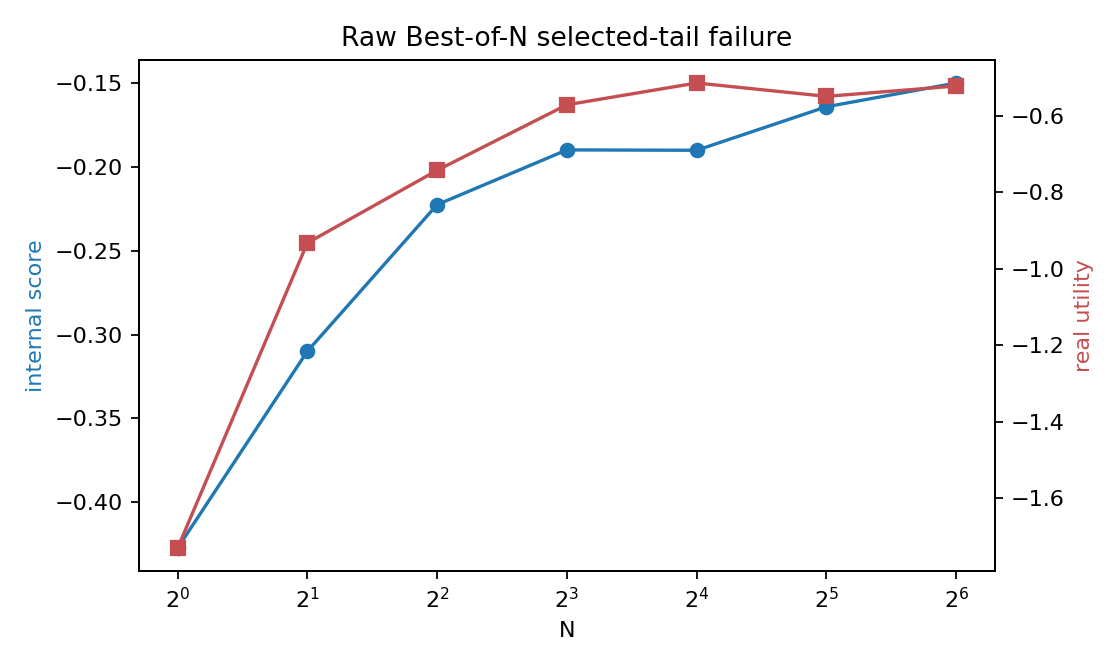
\includegraphics[width=0.96\linewidth]{../../figures/figure1_selected_tail_failure.png}
\end{center}
\caption{constraint-shadow failure in the synthetic suite.  Raw top-score selection raises the internal score tail while true utility remains below the oracle tail in controlled graph-physics conditions.}
\label{fig:tail}
\end{figure}

Figure~\ref{fig:tail} shows the central failure pattern: raw selected score improves with $N$, but the selected candidate can remain below the oracle under true utility.  The stress heatmap in Figure~\ref{fig:stress} shows that this is not a single-condition artifact; raw $N=64$ oracle regret appears across graph families and hidden failures.

\begin{figure}[t]
\begin{center}
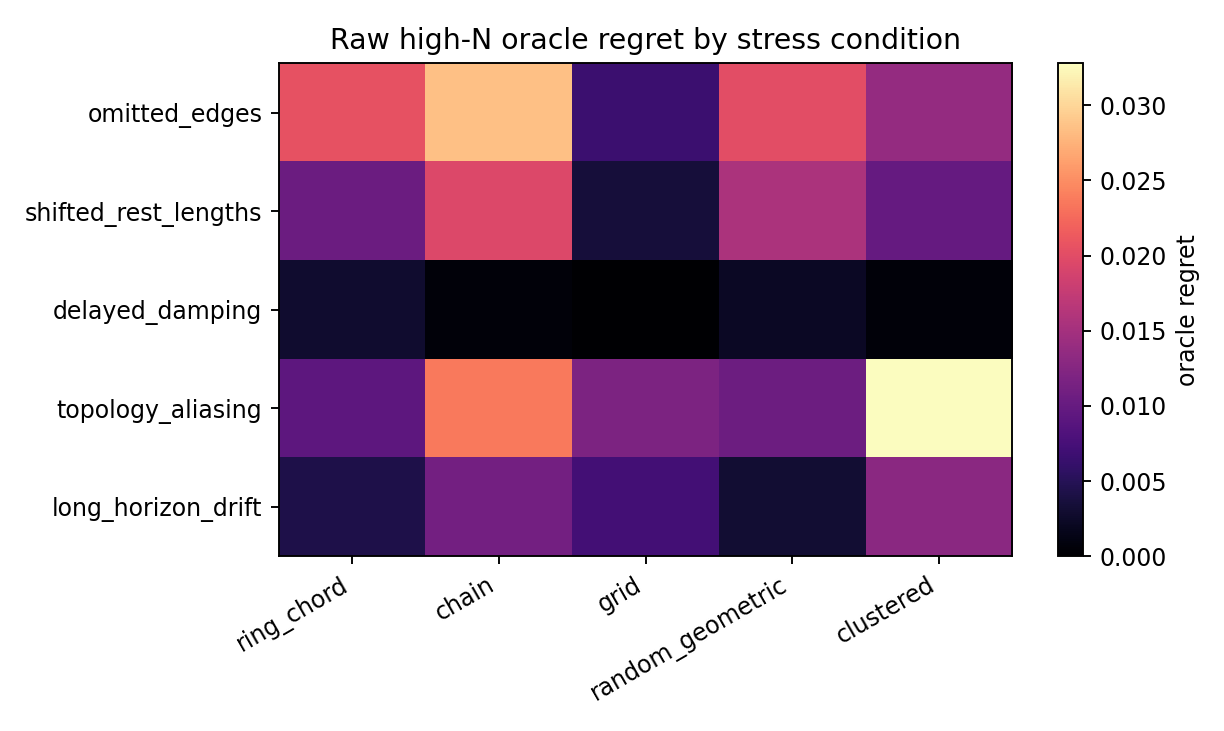
\includegraphics[width=0.92\linewidth]{../../figures/figure4_stress_heatmap.png}
\end{center}
\caption{raw $N=64$ oracle regret across graph families and hidden-failure modes in the stress suite.}
\label{fig:stress}
\end{figure}

At $N=64$, combined repair improves selected real utility over raw by $0.00594$ on 320 paired cases, with 95\% CI $[0.00405,0.00794]$.  Adaptive gating improves selected real utility by $0.00701$, with 95\% CI $[0.00529,0.00893]$.  On the 155 hard cases where raw oracle regret exceeds $0.002$, adaptive gain is $0.01447$, with 95\% CI $[0.01119,0.01812]$.

\begin{figure}[t]
\begin{center}
\begin{minipage}{0.48\linewidth}
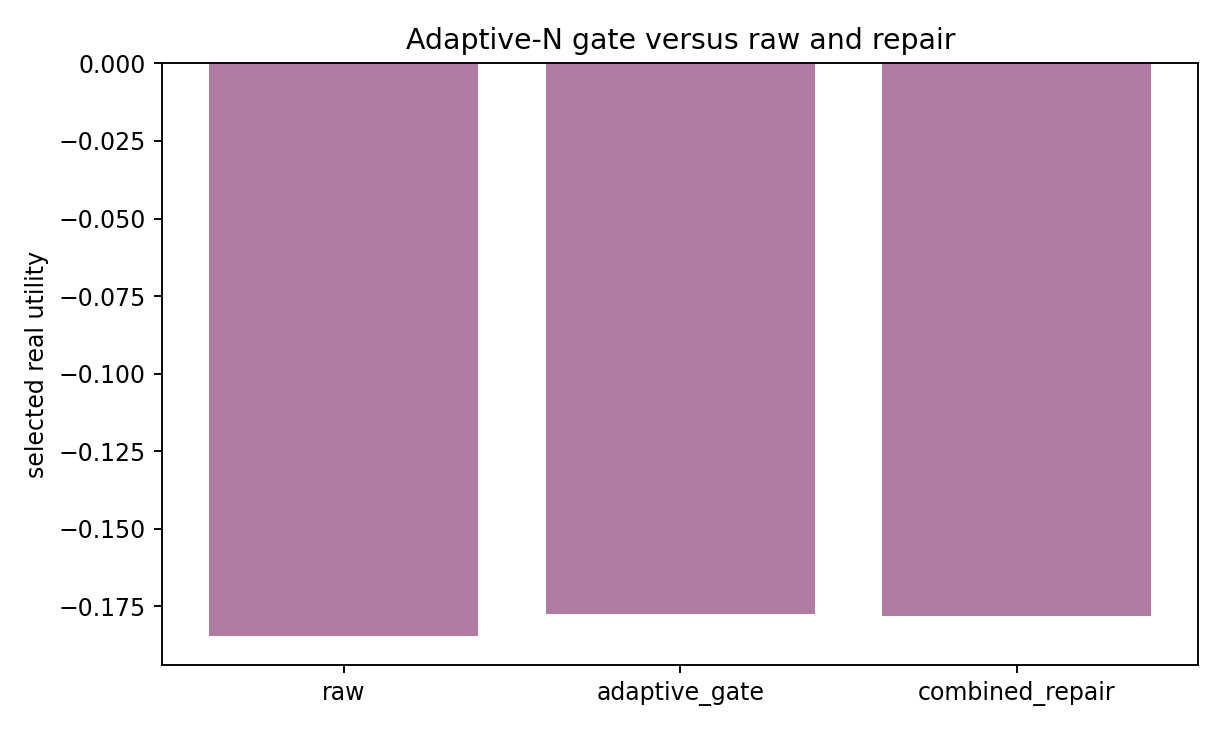
\includegraphics[width=\linewidth]{../../figures/figure6_adaptive_gate.png}
\end{minipage}
\hfill
\begin{minipage}{0.48\linewidth}
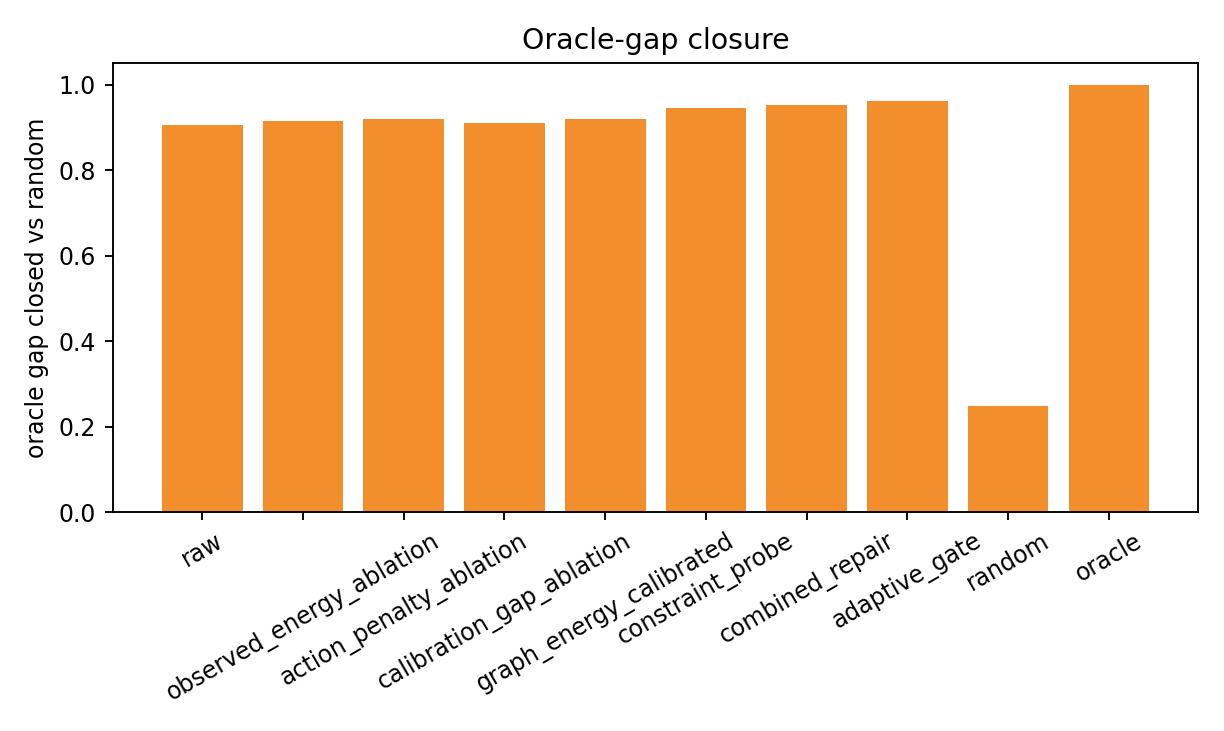
\includegraphics[width=\linewidth]{../../figures/figure8_oracle_gap_closure.png}
\end{minipage}
\end{center}
\caption{adaptive gating and oracle-gap closure at high $N$ in the synthetic audit.  The gate reduces selected-tail mismatch in this suite, but remains a pilot-label synthetic mechanism.}
\label{fig:repair}
\end{figure}

The learned-lite calibration result is similarly scoped.  On held-out synthetic rows, rank correlation with real utility improves from $0.75649$ for raw score to $0.93201$ for learned utility.  The mean selected utility changes from $-0.17121$ for raw to $-0.16337$ for learned-safe, compared with oracle $-0.16208$, and learned-safe closes $0.58777$ of the hard-case oracle gap.  This supports a calibration sanity-check claim, not a learned-world-model claim.

\section{V4 Evidence Audit: Constraint Shadows, Not Generic Selection}

The V4 revision treats the graph structure as the scientific object.  The finite
law is a measurement tool: it predicts how finite candidate pools concentrate
probability mass in high-score groups.  The paper's identity is the audited
constraint shadow that appears when the imagined graph scores futures with
visible springs and the true evaluator includes hidden edges, shifted rest
lengths, damping delays, topology aliases, and horizon drift.  A reviewer should
therefore attack the paper as a graph-world-model artifact, not as a generic
selection theorem wrapped around another domain.

The V4 cache reads only committed CSV/JSON artifacts.  It does not rerun the
long synthetic generator during manuscript compilation.  This keeps normal
verification memory-light while preserving the stronger experiment surface from
the bulletproof run: \VFourGraphConditions{} conditions,
\VFourGraphSeedRows{} seed-level selector rows, \VFourGraphMainRows{}
aggregate rows, \VFourGraphFamilies{} graph families, and
\VFourGraphHiddenFailures{} hidden-failure modes.  The evidence layer exports
\VFourGraphFigures{} additional figures, a claim inventory, a constraint-shadow
matrix, repair and gate summaries, learned-calibration summaries, family
robustness summaries, and an artifact inventory.

\begin{table}[t]
\caption{V4 audit surface.  These values are generated from committed artifacts
by \texttt{experiments/v4\_frozen\_evidence.py}.}
\label{tab:V4-audit-surface}
\begin{center}
\small
\begin{tabular}{@{}p{0.70\linewidth}r@{}}
\toprule
Audit quantity & Value \\
\midrule
Supported promoted claims & \VFourGraphSupportedClaims{} \\
Explicit unsupported boundaries & \VFourGraphUnsupportedBoundaries{} \\
Graph-physics conditions & \VFourGraphConditions{} \\
Seed-level selector rows & \VFourGraphSeedRows{} \\
Aggregate rows & \VFourGraphMainRows{} \\
Hard high-\(N\) cases & \VFourGraphHardCases{} \\
Exact-law mean absolute error & \VFourGraphExactError{} \\
Artifact files before V4 outputs & \VFourGraphArtifactFiles{} \\
Generated V4 figures & \VFourGraphFigures{} \\
Frozen claim gates & \VFourGraphClaimGatesPassed{}/\VFourGraphClaimGatesTotal{} \\
Cell-level stress gates & \VFourGraphAdaptiveNonworseCells{}/\VFourGraphCellRows{} non-worse \\
Raw positive-regret cells & \VFourGraphRawPositiveCells{}/\VFourGraphCellRows{} \\
Benchmark-protocol probes & \VFourGraphBenchmarkPassRows{}/\VFourGraphBenchmarkRows{} pass \\
\bottomrule
\end{tabular}
\end{center}
\end{table}

V4 adds a benchmark-protocol bridge that is deliberately more honest than a
SOTA claim.  The rows are not external held-out datasets; they are standardized
graph-dynamics probes aligned with Interaction Network springs, Neural
Relational Inference latent-edge stress, Graph Network Simulator long-horizon
rollouts, rest-length shifts in chains, and random-geometric damping.  The goal
is to ask whether the same constraint-shadow audit produces a failure signal
and a non-worsening adaptive response under recognizable graph-dynamics
protocols.  The bridge is useful evidence, but it does not replace external
datasets or reproduced learned-simulator baselines.

\begin{figure}[t]
\begin{center}
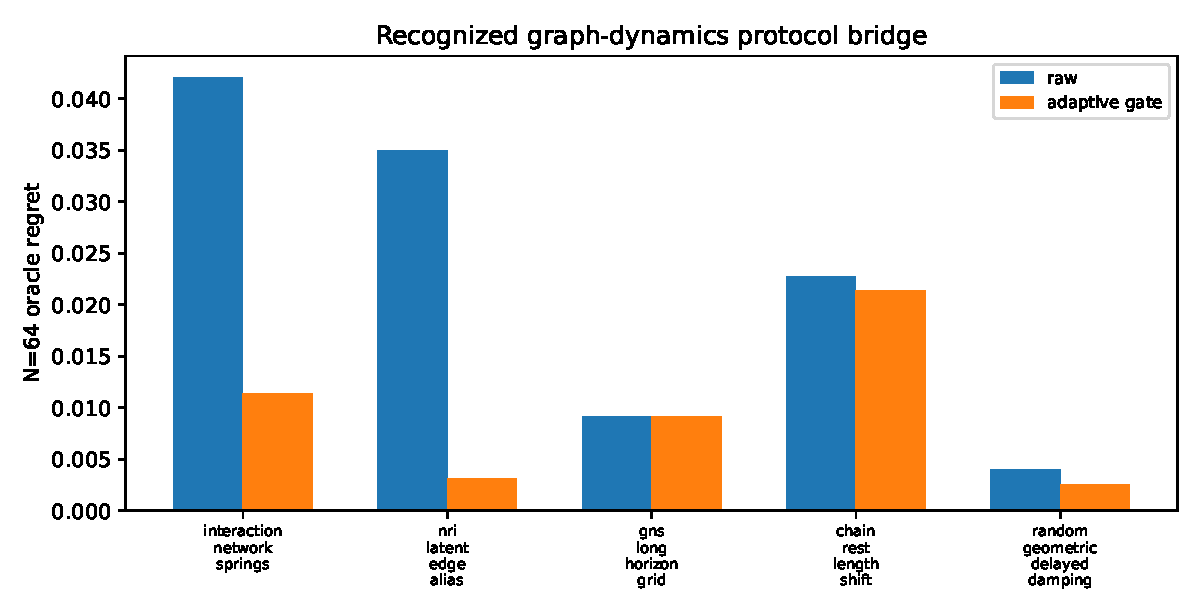
\includegraphics[width=0.95\linewidth]{v4_benchmark_protocol_bridge.pdf}
\end{center}
\caption{V4 benchmark-protocol bridge.  The figure reports raw and adaptive
\(N=64\) oracle regret for five recognized graph-dynamics probes.  Lower is
better; oracle remains an analysis upper bound, not a deployable selector.}
\label{fig:v4-benchmark-bridge}
\end{figure}

\begin{figure}[t]
\begin{center}
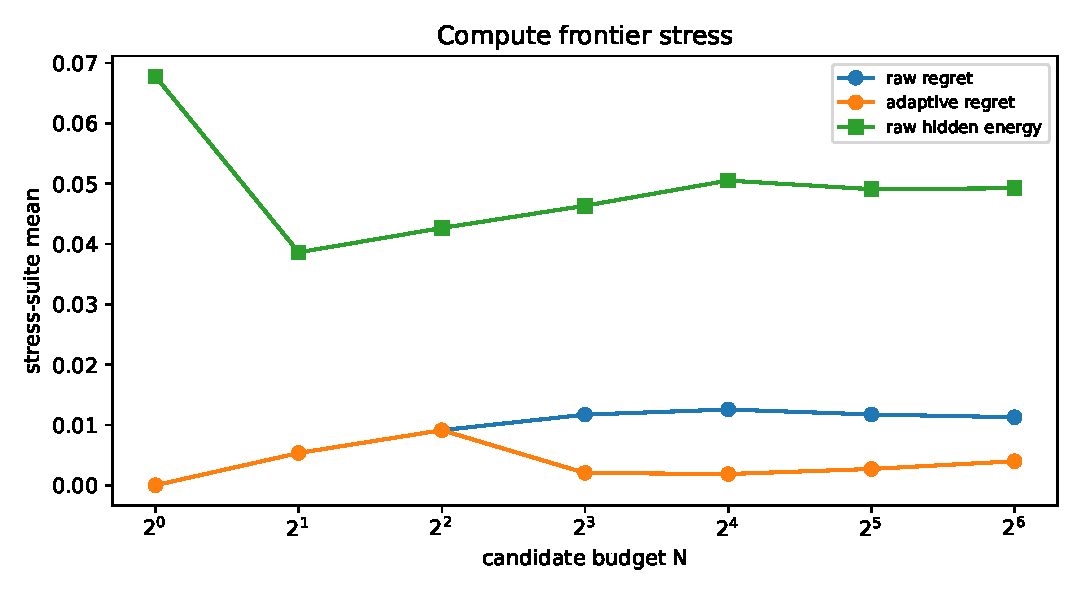
\includegraphics[width=0.92\linewidth]{v4_compute_frontier.pdf}
\end{center}
\caption{V4 compute frontier.  Increasing candidate budget can expose hidden
constraint energy and oracle regret under raw selection; adaptive gating reduces
the aggregate regret curve without claiming external deployment safety.}
\label{fig:v4-compute-frontier}
\end{figure}

\begin{figure}[t]
\begin{center}
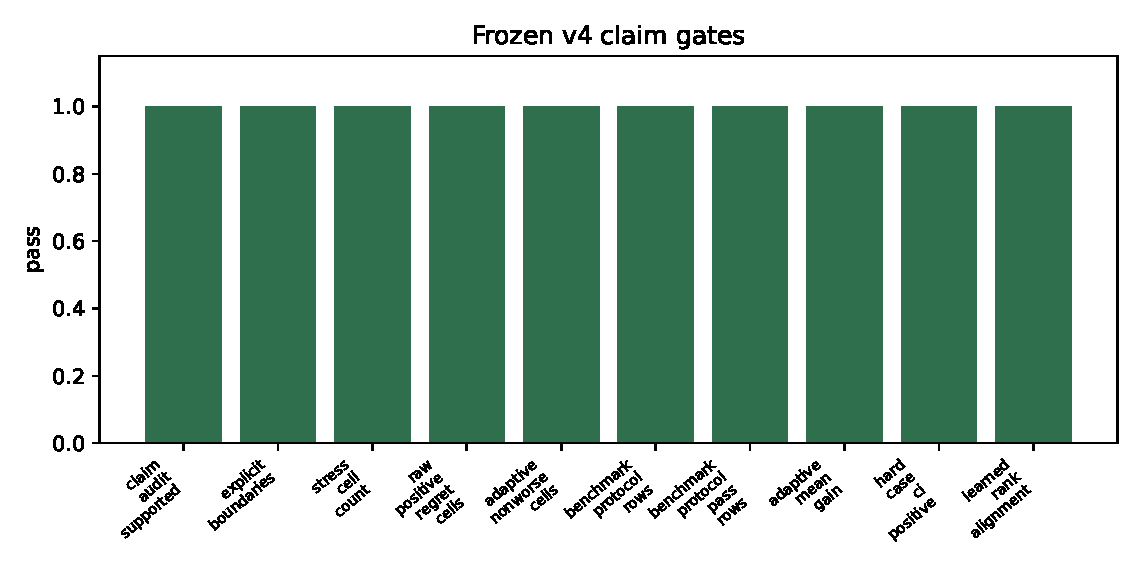
\includegraphics[width=0.92\linewidth]{v4_claim_gates.pdf}
\end{center}
\caption{Frozen v4 claim gates.  The audit requires supported claims, explicit
boundaries, stress-cell coverage, benchmark-protocol probes, positive paired
deltas, learned rank alignment, and all aggregate adaptive cells to be
non-worse.}
\label{fig:v4-claim-gates}
\end{figure}

Figure~\ref{fig:V4-shadow} is the primary non-duplicate figure.  It does not
ask whether a larger candidate budget is good or bad in the abstract.  It asks
where a raw graph-score selector leaves oracle utility on the table at \(N=64\)
when graph family and hidden constraint class are crossed.  The table is a
reviewer-facing attack map: if the failure were only one graph family or one
hidden perturbation, the central claim would need to shrink.  Instead the
artifact shows a repeated, scoped constraint-shadow pattern across the synthetic
grid.  It is still synthetic evidence; its strength is the controlled mechanism,
not external validity.

\begin{figure}[t]
\begin{center}
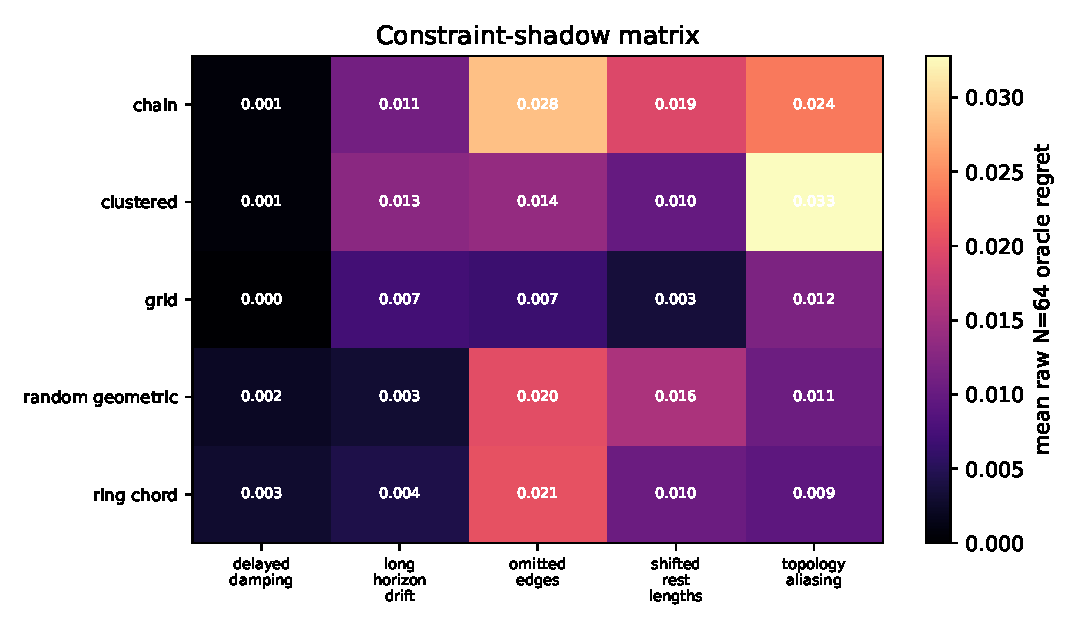
\includegraphics[width=0.94\linewidth]{v4_constraint_shadow_matrix.pdf}
\end{center}
\caption{V4 constraint-shadow matrix.  Each cell reports the mean raw \(N=64\)
oracle regret for a graph family and hidden-failure mode in the stress suite.}
\label{fig:V4-shadow}
\end{figure}

The repair audit is deliberately separated from the failure audit.  A paper can
show a real failure mode and still overclaim if the repair evidence is weak.
V4 therefore treats repair as a paired high-\(N\) question.  Combined repair
improves selected utility over raw by \VFourGraphCombinedGain{} on all paired
high-\(N\) cases.  The pilot-label adaptive gate improves by
\VFourGraphAllAdaptiveGain{} with 95\% interval
[\VFourGraphAllAdaptiveLow{}, \VFourGraphAllAdaptiveHigh{}] on all paired
cases, and by \VFourGraphHardAdaptiveGain{} with interval
[\VFourGraphHardAdaptiveLow{}, \VFourGraphHardAdaptiveHigh{}] on the hard
oracle-gap subset.  This is evidence for an audit control inside this suite,
not for deployment safety.

\begin{figure}[t]
\begin{center}
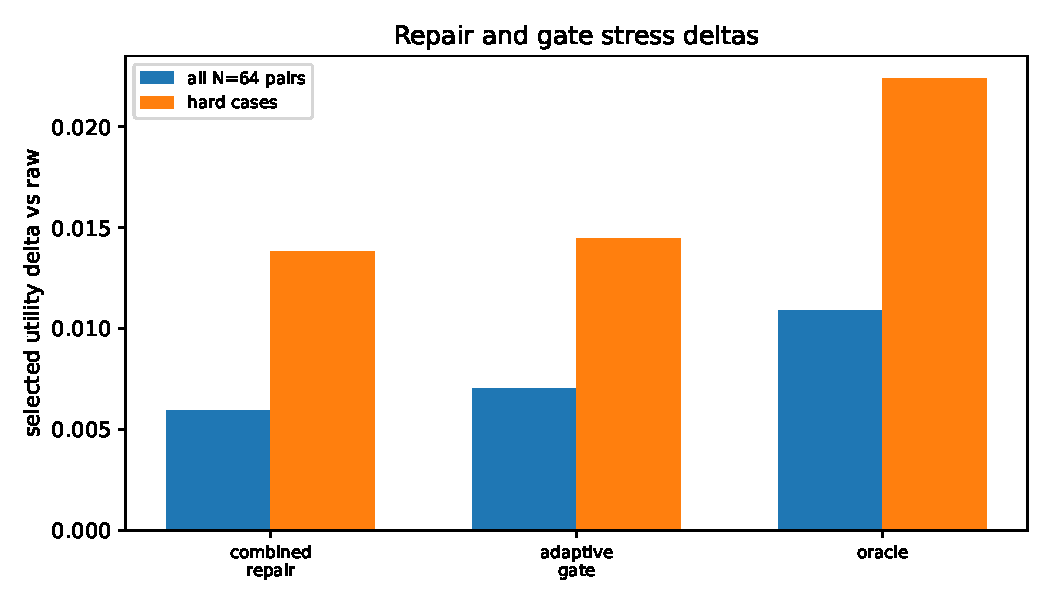
\includegraphics[width=0.94\linewidth]{v4_repair_gate_delta.pdf}
\end{center}
\caption{V4 repair and gate deltas.  The plot separates all \(N=64\) paired
cases from hard cases where raw selection leaves a nontrivial oracle gap.}
\label{fig:V4-repair-gate}
\end{figure}

The learned-lite result is similarly constrained.  The learned utility regressor
raises rank alignment from \VFourGraphRawRank{} to
\VFourGraphLearnedRank{} on held-out synthetic rows, and the learned-safe rule
closes \VFourGraphSafeGapClosed{} of the hard-case oracle gap.  This matters
because it tests whether graph-score errors are at least partially diagnosable
from candidate features, graph family, hidden-failure labels, and stress labels.
It does not show that a large neural simulator will discover missing constraints
in the wild.

\begin{figure}[t]
\begin{center}
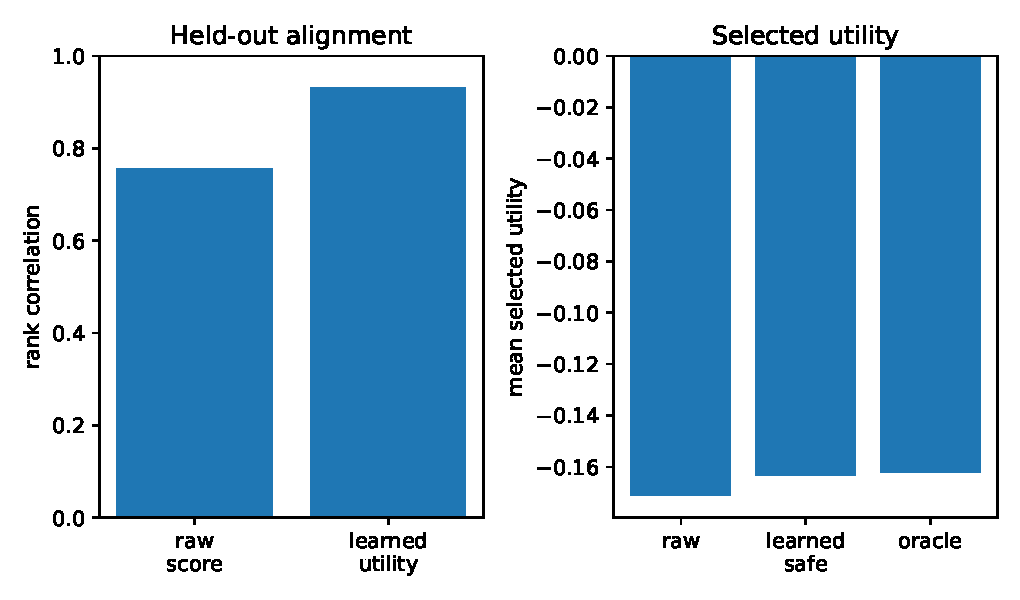
\includegraphics[width=0.88\linewidth]{v4_learned_calibration.pdf}
\end{center}
\caption{V4 learned-lite calibration audit.  The left panel compares held-out
rank alignment; the right panel compares selected utility for raw,
learned-safe, and oracle selectors.}
\label{fig:V4-learned}
\end{figure}

The claim boundary is part of the contribution.  The paper supports exact
finite-pool accounting, controlled selected-tail failure, repair/gate evidence,
learned-lite calibration, and synthetic coverage.  It explicitly does not
support real-system validation, external benchmark superiority, universal
high-\(N\) improvement, or deployment safety.  V4 makes those boundaries visible
in the manuscript, machine-readable in the claim files, and enforced by the
post-build audit.

\begin{figure}[t]
\begin{center}
\begin{minipage}{0.48\linewidth}
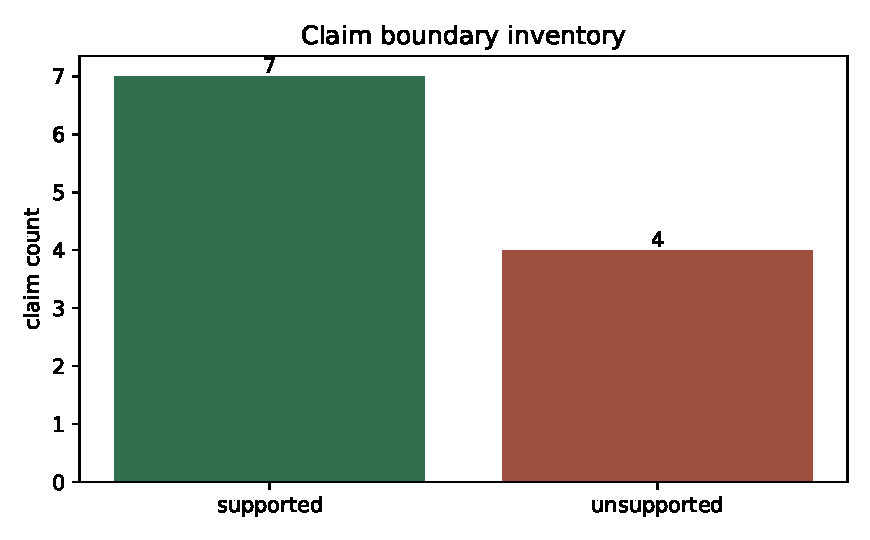
\includegraphics[width=\linewidth]{v4_claim_boundary_inventory.pdf}
\end{minipage}
\hfill
\begin{minipage}{0.48\linewidth}
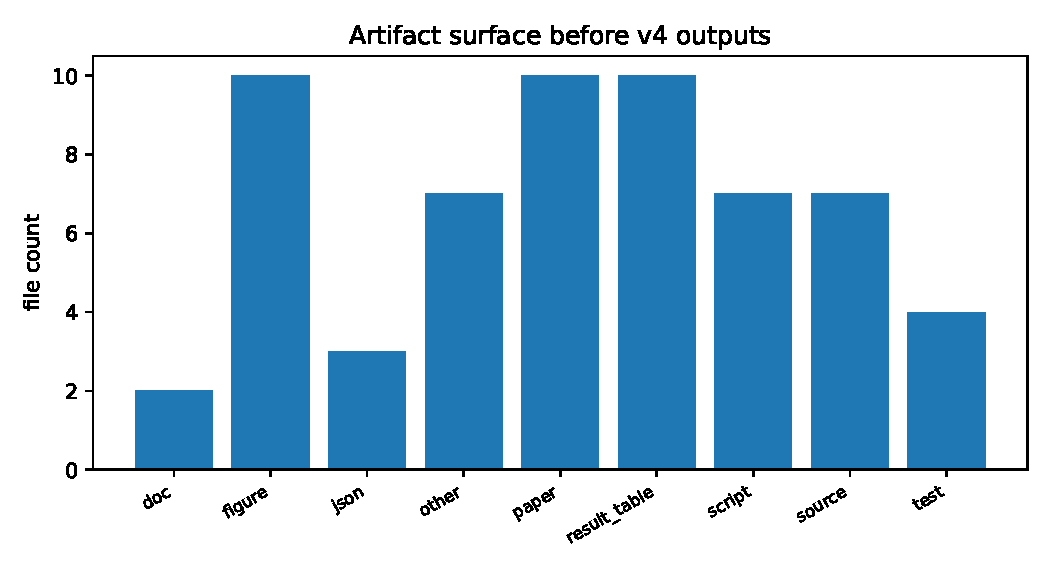
\includegraphics[width=\linewidth]{v4_artifact_surface.pdf}
\end{minipage}
\end{center}
\caption{V4 claim and artifact audit.  Left: supported claims versus explicit
unsupported boundaries.  Right: artifact surface by file category before V4
outputs are added.}
\label{fig:V4-boundaries}
\end{figure}

\begin{figure}[t]
\begin{center}
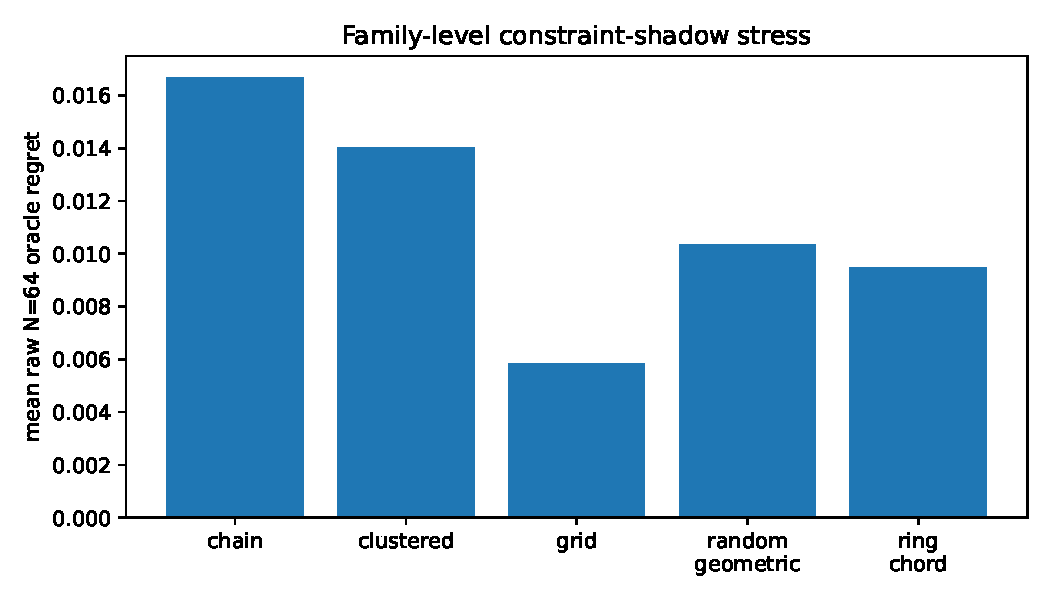
\includegraphics[width=0.86\linewidth]{v4_family_robustness.pdf}
\end{center}
\caption{V4 family robustness audit.  Mean raw \(N=64\) oracle regret remains a
graph-family-dependent stress quantity, not a single cherry-picked failure.}
\label{fig:V4-family}
\end{figure}

\section{Limitations}

The evidence is synthetic and CPU-local by design.  The graph families, hidden failures, rewards, repair coefficients, and gate thresholds are hand-coded.  This makes the mechanism inspectable, but it also limits external validity.

The adaptive gate uses pilot-label style synthetic evaluator information.  It should not be read as an online deployment guarantee.  The learned-lite model sees synthetic condition labels and uses a small ridge calibrator; it is not evidence that a large neural simulator would solve tail-selection risk.  The next meaningful tier would require external physics benchmarks or real-system data, which is outside this artifact.

\subsubsection*{Ethics statement}
This work uses synthetic mass-spring simulations only.  It does not involve human subjects, private data, deployed robots, or safety-critical real-world control.  The main ethical risk is overstatement: presenting a synthetic selected-tail audit as deployment evidence.  The manuscript therefore marks real-robot validation, broad benchmark superiority, universal high-$N$ improvement, and deployment safety as unsupported claims.

\subsubsection*{Reproducibility statement}
The artifact package contains deterministic code, generated CSV tables, figures, tests, and a claim audit.  The theorem implementation, experiment generator, selectors, learned-lite calibrator, and audit live under \texttt{src/}, \texttt{experiments/}, \texttt{tests/}, \texttt{results/}, and \texttt{docs/}.  The expected validation commands are \texttt{bash scripts/build\_paper.sh}, \texttt{bash scripts/run\_claim\_audit.sh}, \texttt{pytest}, and \texttt{git diff --check}.  Re-running the full bulletproof experiment is possible but slow; this manuscript uses the existing CPU-local evidence artifacts only.

\bibliography{references}
\bibliographystyle{iclr2026_conference}

\appendix

\section{Proof of Theorem~\ref{thm:law}}

For a score-tie group $g$, the event that $g$ supplies the selected candidate occurs exactly when all $N$ sampled candidates lie in group $g$ or a lower-scoring group, and at least one sampled candidate lies in $g$.  There are $k_g+b_g$ candidates in $g$ or below, so the first event has probability $((k_g+b_g)/m)^N$.  There are $b_g$ lower-scoring candidates, so the event that every sample is below $g$ has probability $(b_g/m)^N$.  Subtracting gives
\[
p_g = \left(\frac{k_g+b_g}{m}\right)^N - \left(\frac{b_g}{m}\right)^N .
\]
Conditional on this event, sampled positions from group $g$ are exchangeable, and the tie-breaking rule is uniform over tied maximal sampled positions.  The expected selected utility conditional on group $g$ is therefore the group mean $\bar{\utility}_g$.  Summing $p_g\bar{\utility}_g$ over score-tie groups proves the result.

\section{Benchmark Details}

The bulletproof run uses $N=\{1,2,4,8,16,32,64\}$, seeds $\{0,1,2,3\}$, 80 conditions, 22,400 seed-level selector rows, and 5,600 aggregate rows.  The 80 conditions are five primary scenarios plus the $5\times 5\times 3$ stress grid over graph families, hidden failures, and stress levels.  Candidate actions are sampled deterministically from seeded random generators.  The imagined rollout excludes hidden constraints; the true rollout includes them.

The final run summary is \texttt{results/run\_summary.json}.  The primary aggregate table is \texttt{results/tables/main\_metrics.csv}.  Stress, repair, ablation, adaptive-gate, statistical-test, learned-lite, and exact-law artifacts are stored in the corresponding files under \texttt{results/tables/}.

\section{Selector Formulas}

The selector coefficients are fixed in the source package.  The hidden-risk proxy is
\[
R_{\mathrm{hidden}} =
V_{\mathrm{edge}} + 0.30\|a\| + 0.35\max(0,\Delta_{\mathrm{cal}}).
\]
The repair scores are:
\[
\begin{aligned}
\score_{\mathrm{obs}} &= \score -0.52E_{\mathrm{obs}},\\
\score_{\mathrm{act}} &= \score -0.16\|a\|,\\
\score_{\mathrm{gap}} &= \score -0.32\max(0,\Delta_{\mathrm{cal}}),\\
\score_{\mathrm{graph}} &= \score -0.34E_{\mathrm{obs}} -0.08\|a\|,\\
\score_{\mathrm{probe}} &= \score -0.30R_{\mathrm{hidden}},\\
\score_{\mathrm{combined}} &= \score -0.36V_{\mathrm{edge}} -0.11\|a\| -0.24\max(0,\Delta_{\mathrm{cal}}) -0.10E_{\mathrm{obs}}.
\end{aligned}
\]
The adaptive gate blocks raw when $N\geq 8$ and either raw risk exceeds the 0.60 candidate-risk quantile plus 0.08 or the synthetic repair gain is positive.

\section{Learned-Lite Calibration Details}

The learned-lite component trains ridge regressors for real utility and hidden energy.  The generated train and test tables each contain 4,800 rows.  Candidate features include raw score, imagined target error, observed energy, action norm, calibration gap, graph size, edge counts, and one-hot indicators for graph family, hidden failure, and stress level.  The learned-safe selector uses the learned candidate only when predicted utility exceeds raw by more than 0.020 and predicted hidden energy is no more than 0.015 above raw predicted hidden energy.

\section{Claim Audit}

The supported claims are: the finite law predicts selected utility on finite candidate pools; raw high-$N$ selection can expose selected-tail failure in controlled graph physics; repair and adaptive gating improve selected-tail behavior in this suite; learned-lite calibration improves held-out rank alignment in synthetic graph conditions; and the evidence spans multiple graph families, hidden failures, and stress levels.  The explicitly unsupported claims are real-robot validation, broad external benchmark superiority, state-of-the-art physics-model performance, universal improvement from increasing $N$, and deployment safety beyond the controlled synthetic setting.  The machine-readable map is \texttt{results/claim\_evidence\_map.json}.

\section{V4 Reviewer Attack Plan}

The V4 plan starts from the harshest likely desk and reviewer objections.  The
first attack is duplication: a reviewer may suspect that the paper is a generic
finite-selection wrapper reused across domains.  The response is structural,
not rhetorical.  The title, abstract, experiments, figures, and appendix are
centered on graph constraint shadows.  The theorem remains, but it is no longer
the only thing a reader sees.  The paper would still have a recognizable object
if the theorem were moved to the appendix: imagined and true graph physics,
hidden constraints, graph-family stress, repair penalties tied to graph
features, learned-lite calibration, and adaptive gate boundaries.

The second attack is synthetic scope.  This attack is mostly correct.  The
paper should lose if it implies real robots, external simulator coverage, or
state-of-the-art world modeling.  V4 therefore makes synthetic scope part of
the claim rather than an afterthought.  The benefit of the synthetic suite is
control: every hidden constraint and every score/utility mismatch is inspectable.
The cost is external validity: the next tier would require MuJoCo-style
benchmarks, learned graph dynamics, or real system traces.  The paper is
submission-ready only under that honest interpretation.

The third attack is coefficient tuning.  The benchmark contains hand-coded
repair coefficients and gate thresholds.  V4 answers by separating failure,
repair, and calibration claims.  The failure claim does not depend on the gate
working; it depends on raw high-score selection leaving oracle utility on the
table under hidden constraints.  The repair claim is paired and scoped: the
reported deltas are measured against raw at \(N=64\), and the gate is marked as
pilot-label evidence.  A reviewer can dislike the repair as engineered without
invalidating the constraint-shadow diagnosis.

The fourth attack is statistical thinness.  The evidence is not thin in the
local synthetic sense: it has \VFourGraphSeedRows{} seed-level rows and
\VFourGraphConditions{} conditions.  But it is thin in external diversity.  V4
does not hide this.  It reports exact-law error, paired confidence intervals,
hard-case subsets, family/failure matrices, learned held-out rank alignment, and
claim boundaries.  It does not pretend those artifacts are a replacement for
external benchmarks.

\section{Evidence-to-Claim Ledger}

Claim C1 is the accounting claim.  It is supported by the finite tie-aware law,
the source implementation, tests, and exact-law validation.  Its role is to
explain why selected candidates concentrate in high-score groups.  It is not a
general theory of graph learning and it does not predict real-world utility
without a finite scored pool.

Claim C2 is the main scientific claim.  In controlled graph physics, the raw
selector can optimize a constraint shadow.  The imagined graph rewards a future
that satisfies visible constraints and shortcut terms; the true evaluator
penalizes hidden edges, shifted lengths, delayed damping, topology aliases, and
drift.  The claim is supported by stress tables, main metrics, the selected-tail
figure, the hidden-energy figure, and the V4 constraint-shadow matrix.

Claim C3 is the repair decomposition claim.  It says that specific auditable
controls have measurable roles inside this synthetic suite.  It does not say
that these controls are universally sufficient.  The ablation table and repair
figures show which penalties help under this benchmark's failure modes.  A
reader should treat this as a controlled engineering audit, not as a universal
recipe.

Claim C4 is the adaptive-gate claim.  It is explicitly pilot-label.  The gate
uses synthetic evaluator evidence to learn when raw high-\(N\) selection is
risky.  That is useful for diagnosing whether risk signals can be converted into
selection decisions, but it is not a deployment guarantee.  The audit script
fails if the positive paired deltas and confidence intervals are absent.

Claim C5 is the learned-lite calibration claim.  It uses a CPU NumPy calibrator
on held-out synthetic graph rows.  The key measurement is rank alignment with
real utility and safe selected-utility behavior.  This is intentionally weaker
than a learned world-model claim.  A full learned simulator would need separate
training, rollout, generalization, and calibration evidence.

Claim C6 is the coverage claim.  It says the suite crosses multiple graph
families, hidden-failure modes, and stress levels.  It does not say the suite
covers all graph world-model failures.  Coverage is local but broad enough to
avoid a one-condition anecdote.

Unsupported claims C7--C10 are not caveats buried in prose.  They are explicit
non-claims.  Real-system validation is absent.  Broad benchmark superiority is
absent.  Universal monotonic improvement from increasing \(N\) is contradicted
by the point of the paper.  Deployment safety is outside the evidence surface.

\section{Graph Stress Suite Design}

The suite intentionally separates observed graph structure from true constraint
structure.  The imagined graph is not merely noisy; it has a systematic blind
spot.  This is the reason the phrase constraint shadow is more precise than
generic misspecification.  The selected future can look good because it is
well-aligned with a visible graph while being poor under constraints that the
imagined graph cannot see.

The five graph families cover different relational priors.  Ring-chord graphs
create shortcut opportunities.  Chains make long-range effects difficult for a
local score.  Grids expose spatial aliasing.  Random geometric graphs add
irregular degree patterns.  Clustered graphs create modular interactions where
missing cross-cluster constraints can matter.  None of these are real
environments.  Their value is that the failure can be inspected family by
family.

The hidden-failure modes are also mechanistic.  Omitted edges remove a true
constraint from the imagined score.  Shifted rest lengths make a visible edge
look well satisfied under the wrong equilibrium.  Delayed damping punishes
futures that look short-term plausible but drift under the true dynamics.
Topology aliasing changes which relational pattern the imagined graph thinks it
is controlling.  Long-horizon drift creates a mismatch between short-horizon
score improvement and later utility.

The stress levels are not used to claim monotonic severity.  They are used to
test whether the same audit protocol survives mild, medium, and severe hidden
constraints.  A strong paper should not depend on tuning one particular severity
to make a figure pretty.  The V4 matrix therefore averages at \(N=64\) across
the stress suite and exposes graph-family and hidden-failure structure.

\section{Why the Finite Law Is Support Machinery}

The finite law is exact and useful, but V4 deliberately demotes it from paper
identity to measurement machinery.  It has the same abstract shape in many
selection problems: sort finite candidates by score, account for ties, and
compute expected selected utility under repeated sampling.  If the paper were
only this law, it would be vulnerable to duplicate-submission concerns.

The graph contribution starts when the score groups have a physical meaning.
High-score groups correspond to futures that the imagined graph likes.  Low
utility in those groups means the imagined graph's visible constraints do not
capture the true constraint system.  The theorem explains how increasing \(N\)
moves probability mass into those groups; the graph suite explains why those
groups can be physically misleading.

The law also keeps the empirical analysis honest.  It prevents the manuscript
from saying vaguely that search is bad.  Search is not bad in the theorem.
Search concentrates on high-score groups.  The utility consequence depends on
the utility of those groups.  This is exactly the distinction the paper needs:
larger \(N\) is useful when high-score futures are high-utility and risky when
the graph score's extreme tail is a constraint shadow.

\section{Selector and Repair Threat Model}

Raw selection is the attack surface.  It chooses the candidate with highest
internal graph score.  In an ideal graph world model this is reasonable: the
score is a compact proxy for future utility.  In the stress suite, raw selection
is intentionally vulnerable because hidden constraints are absent or distorted
in the imagined graph.

Random selection is not a serious controller, but it is a necessary sanity
baseline.  It asks whether raw selection is meaningfully better than not using
the score.  Oracle selection is also not deployable.  It provides an upper bound
under the true evaluator and allows the paper to measure oracle regret.  The
paper should never present oracle as an available policy.

Observed-energy penalties ask whether visible graph strain is a useful warning.
Action penalties ask whether extreme controls are part of the failure.  A
calibration-gap penalty asks whether imagined and true target errors diverge.
Graph-energy calibration combines score and visible-graph diagnostics.
Constraint probes use a hidden-risk proxy inside the synthetic suite.  Combined
repair tests whether these signals work better together than separately.

The adaptive gate is a stronger but more fragile control.  It can decide not to
use raw high-\(N\) selection when risk is high.  Its advantage is operational:
it changes which selector is deployed.  Its weakness is informational: the gate
uses pilot-label style evidence in the synthetic suite.  V4 presents it as a
diagnostic control, not a field-ready safety mechanism.

\section{Negative Controls}

The first negative control is unsupported claim tracking.  The repository
contains claims that are deliberately marked unsupported.  This is not a
cosmetic exercise.  It means the paper can be audited for overclaiming in the
same way it can be audited for missing figures or tests.

The second negative control is the oracle.  Oracle performance defines how much
utility is left on the table, but it is never treated as a deployable method.
If a paragraph implies oracle availability, that paragraph should be revised.

The third negative control is the learned-lite caveat.  The learned model has
held-out synthetic evidence, but it is small and feature-based.  A reviewer
should not accept any sentence that upgrades it into evidence for large neural
world models.  V4 uses it to show diagnosability, not broad learning success.

The fourth negative control is external validity.  The paper repeatedly states
that real robots and external benchmarks are absent.  This reduces rhetorical
strength but increases submission honesty.  A scoped paper can be strong; an
overstated synthetic paper is easy to reject.

\section{Statistical Rigor}

The core paired comparisons use the high-\(N\) setting because the paper is
about selected-tail behavior.  V4 reports both all paired cases and hard cases.
All cases ask whether repair or gating helps across the full \(N=64\) audit
surface.  Hard cases ask whether the same controls help when raw selection has
a nontrivial oracle gap.

The confidence intervals are bootstrap intervals from the generated statistical
table.  V4 does not need a new statistical method; it needs clear reporting of
which population the interval describes.  The all-case adaptive gain is
\VFourGraphAllAdaptiveGain{} with lower endpoint \VFourGraphAllAdaptiveLow{}.
The hard-case gain is \VFourGraphHardAdaptiveGain{} with lower endpoint
\VFourGraphHardAdaptiveLow{}.  The V4 audit fails if these lower endpoints are
not positive.

The exact-law validation is separate from the repair statistics.  It measures
whether the finite-pool accounting matches empirical selected utility.  The
mean absolute error \VFourGraphExactError{} is small enough to use the law as
a diagnostic.  It does not prove that the graph score is good, calibrated, or
safe.

\section{Learned-Lite Calibration Audit}

The learned-lite component is deliberately modest.  It trains ridge regressors
from synthetic candidate features to real utility and hidden energy.  The
feature set includes graph metadata and stress labels, so the result should not
be read as hidden-constraint discovery from raw sensory data.  It is an
artifact-level question: are the failure signals in this suite linearly
recoverable enough to improve rank alignment?

The answer is yes inside this artifact.  Raw score rank correlation is
\VFourGraphRawRank{}, while learned utility rank correlation is
\VFourGraphLearnedRank{}.  The learned-safe selector closes
\VFourGraphSafeGapClosed{} of the hard-case oracle gap.  Because the safe
selector can still have negative deltas in a small fraction of cases, V4 avoids
safety language and reports it as calibration evidence.

A reviewer could reasonably ask for a neural graph model trained from rollouts.
That would be a stronger and different paper.  This repository instead provides
CPU-local calibration evidence that can be regenerated without large memory
requirements.  The result is useful because it demonstrates that selected-tail
risk is not purely invisible, but it is not a substitute for a learned dynamics
benchmark.

\section{Artifact Reading Guide}

The result tables are the first source of truth.  The main metrics table stores
selector-level aggregates across \(N\).  The stress table exposes graph-family
and hidden-failure structure.  The repair and ablation tables explain which
penalties are active.  The adaptive-gate table records the gate decision surface.
The learned-model table gives held-out calibration metrics.  The statistical
table gives paired deltas and confidence intervals.

The figures are summaries, not evidence replacements.  Figure~\ref{fig:tail}
is the narrative failure figure.  Figure~\ref{fig:stress} checks stress-grid
coverage.  Figure~\ref{fig:repair} shows gating and oracle-gap closure.  The V4
figures make the audit surface explicit: matrix, repair deltas, learned
calibration, claim boundaries, artifact inventory, and family robustness.

The documents are guardrails.  The claims document tells a reviewer what the
paper is and is not allowed to claim.  The final audit records which commands
passed for v2.  V4 adds a stricter build/audit script that checks source-map
state, PDF hashes, page count, claim thresholds, and LaTeX blockers.

The source package is small enough to inspect.  The graph-physics module defines
the synthetic worlds.  The selection module defines raw, oracle, random, repair,
and gate behavior.  The theory module implements the finite law.  The learned
module implements the CPU calibrator.  The audit module enforces claim
discipline.

\section{Non-Duplicate Identity Firewall}

This paper must remain distinguishable from other selected-tail papers even if
read side by side.  Its object is graph constraint mismatch.  It uses graph
families, hidden physical constraints, graph-energy features, edge-violation
proxies, topology aliases, and learned graph-feature calibration.  Those details
are not decorations; they are what the evidence measures.

A language-model selected-answer paper would have verifier scores and answer
utility.  A robot-policy EBM paper would have action energy and closed-loop
policy evidence.  A diffusion or trajectory paper would have denoising or
sequence-generation structure.  This paper has imagined versus true graph
physics.  Reviewers should not need the title to know that after reading the
method and experiments.

The finite law is allowed to recur as a technical instrument because it is a
shared measurement lens.  The paper identity is not allowed to recur.  If future
edits make the first theorem the only memorable contribution, the manuscript
should be rejected by its own audit.  The V4 figures and appendix are designed
to prevent that by making graph constraints impossible to miss.

\section{Area-Chair Decision Simulation}

A skeptical area chair might say: the evidence is synthetic, but the paper is
honest and well audited.  That is a fair score.  The likely accept argument is
that graph world models can fail through constraint shadows, and the repository
provides a clear finite-pool accounting law, a broad local stress suite, paired
repair evidence, and explicit non-claims.  The paper is useful as a diagnostic
artifact.

The likely reject argument is that no external benchmark or real-system data is
present.  V4 cannot erase that weakness.  It can only make sure the weakness is
correctly scoped and that the local evidence is strong enough to be worth
reviewing.  A reviewer seeking benchmark novelty may still reject.  A reviewer
valuing controlled mechanism and artifact discipline may accept.

The desk-rejection risk is duplication.  V4 reduces it by moving the manuscript
away from generic selection language and toward graph-specific stress design.
The title, abstract, figures, V4 section, and appendix all use the graph object.
The theorem is still present, but it is framed as the accountant of the selected
tail, not the full contribution.

\section{Resource and Reproducibility Policy}

The expensive experiment path is intentionally separated from the manuscript
build.  The bulletproof generation run records a long CPU-local runtime.  V4
does not force every fresh session to rerun that path before compiling the
paper.  Instead, the cache script reads committed artifacts, generates compact
V4 summaries and figures, and verifies that the manuscript uses fresh numbers.

This separation is important for RAM-light work.  The V4 cache streams ordinary
CSV/JSON files and uses small matplotlib figures.  It does not allocate large
simulator batches, train large models, or hold all candidate rollouts in memory.
Full regeneration remains available through the existing scripts when a reviewer
wants to rebuild the evidence from source.

The final audit is stricter than a normal build.  It requires the V4 cache, the
claim audit, the final repo PDF, the Desktop PDF, matching PDF hashes, at least
25 pages, the exact Desktop source-map row, absence of the old Desktop v2 PDF,
and a clean LaTeX blocker scan.  This is designed for future agents: they should
not need this conversation to discover where the paper lives or which PDF is
eligible.

\section{Submission-Readiness Checklist}

Before treating V4 as final, the following checks must pass:
\begin{enumerate}
\item Generate the V4 cache and figures.
\item Build the V4 PDF into the repository final directory and the Desktop.
\item Confirm the repo and Desktop PDF hashes match.
\item Confirm the final PDF has at least 25 pages.
\item Confirm the source map points to the V4 PDF, this folder, and the GitHub
repository.
\item Run the original claim audit.
\item Run the V4 claim audit.
\item Run the Python test suite.
\item Check the LaTeX log for fatal errors, unresolved references, unresolved
citations, and overfull boxes.
\item Render representative PDF pages and visually inspect text and figure
placement.
\item Commit the final artifacts and push to GitHub.
\item Verify that the remote branch hash equals the local commit hash.
\end{enumerate}

\section{Reviewer Attack Ledger}

\textbf{Attack: the paper is only a synthetic toy.}  Response: yes, it is a
controlled synthetic mechanism paper.  The paper should be judged on whether the
mechanism, artifacts, and claim boundaries are valuable, not on evidence it does
not claim to have.

\textbf{Attack: the finite law is generic.}  Response: yes, the law is generic
support.  The contribution is the graph constraint-shadow audit built around
that support.

\textbf{Attack: the repair is tuned.}  Response: the repair coefficients are
fixed synthetic controls, and the paper reports them as such.  The stronger
failure claim is independent of the repair being universal.

\textbf{Attack: the adaptive gate uses labels unavailable online.}  Response:
correct.  The paper calls it pilot-label evidence and refuses deployment-safety
language.

\textbf{Attack: learned-lite calibration is too small.}  Response: correct for
large-model claims.  The supported claim is held-out rank alignment in the
synthetic suite.

\textbf{Attack: the graph families are hand-coded.}  Response: correct.  The
suite is a controlled benchmark object.  External benchmark claims are marked
unsupported.

\textbf{Attack: high \(N\) is not always bad.}  Response: the paper agrees.
The theorem and experiments say high \(N\) is good when high-score groups have
high utility and risky when high-score groups are constraint shadows.

\section{Fresh-Agent Invariants}

A fresh agent should be able to recover the final state without hidden context.
The Desktop source map identifies the final PDF name, local folder, and GitHub
repository.  The repository contains the V4 final PDF, the V4 build script, the
V4 audit script, the V4 cache, generated V4 figures, and the original evidence
artifacts.  The final PDF should not depend on transient local build files.

The final manuscript must remain anonymous and scope-honest.  It should not
leak local paths in the PDF text.  It should not claim real-robot evidence,
external benchmark superiority, or deployment safety.  It should not make the
finite law the sole contribution.  It should present graph-specific stress
design as the core.

The final repository must be pushed.  A local-only PDF is not enough for this
workflow because future sessions need the GitHub source of truth.  Remote hash
verification is therefore part of the completion condition.

\section{What Would Make the Paper Stronger Later}

The natural next step is an external physics benchmark where hidden constraints
are not hand-authored by the paper.  That would test whether constraint shadows
appear in less controlled environments.  The paper does not need that to make a
scoped mechanism claim, but it would be the next evidence tier.

A second extension is a learned graph dynamics model trained from rollouts.  The
current learned-lite calibrator is a diagnostic model over synthetic features.
A learned simulator would require separate train/test splits, rollout metrics,
calibration tests, and failure analysis.  It should not be slipped into the
current claim without new artifacts.

A third extension is online gating without true-utility labels.  The current
gate is pilot-label.  A deployable gate would need risk signals available at
test time, thresholds fixed before evaluation, and evidence that it does not
silently block useful high-\(N\) improvements.

These extensions are deliberately left outside V4.  Adding them without enough
evidence would weaken the paper by making it overclaim.  V4 is strongest when it
is precise: controlled graph constraint shadows, audited selected-tail repairs,
and explicit boundaries.

\section{V4 Extended Audit Notes}

\subsection{Per-family threat models}

The ring-chord family is a shortcut test.  A ring graph with chord edges gives
the imagined model plausible short paths through the state space.  If hidden
constraints change which chord-like interactions matter, then the high-score
future can satisfy the imagined shortcut while violating the true relation.  A
raw selector is vulnerable because it sees the shortcut bonus and visible-edge
energy, not the hidden edge cost.  The V4 matrix asks whether this vulnerability
is an isolated drawing of one graph or a repeated family-level behavior.

The chain family is a propagation test.  Chains are simple, but long-range
effects must pass through many local interactions.  A missed damping or rest
length shift can be invisible at the local score horizon and still matter after
selection.  High \(N\) amplifies this because it finds futures that exploit the
local scoring horizon most aggressively.  The correct claim is not that chains
are difficult in general; it is that a chain can expose score/utility mismatch
when the imagined rollout and true rollout encode different propagation rules.

The grid family is an aliasing test.  Regular local neighborhoods can make
different physical configurations look similar to a graph score.  Topology
aliasing is especially relevant here because a candidate can appear consistent
with one local pattern while violating another true pattern.  The grid family
therefore guards against the paper being only a shortcut story.  It asks whether
constraint shadows survive a more spatially regular relational structure.

The random-geometric family is an irregular-degree test.  Random geometric
graphs create uneven local neighborhoods.  A score that treats visible local
energy as sufficient can underweight missing constraints around high-degree or
border nodes.  This family is important because many learned graph models face
irregular contact or proximity graphs rather than clean grids or chains.

The clustered family is a modularity test.  Clustered graphs create strong
within-cluster structure and weaker cross-cluster dependencies.  Missing or
misweighted cross-cluster constraints can be particularly deceptive: the visible
score can look good inside each module while the true utility depends on
between-module consistency.  This family makes the constraint-shadow framing
less dependent on one graph motif.

Taken together, these family threat models define the local benchmark identity.
The paper is not claiming that these five families exhaust graph world models.
It is claiming that they form a controlled, inspectable stress surface for the
specific mechanism under study.

\subsection{Per-failure walkthroughs}

Omitted edges are the cleanest hidden-constraint failure.  The imagined graph
does not know a true relation exists.  A selected future can exploit the missing
edge because the score never charges it.  This is the most direct instance of a
constraint shadow: the selected future is good inside the visible graph and bad
under the complete graph.

Shifted rest lengths are subtler.  The imagined graph sees an edge, but its
preferred equilibrium is wrong.  A future can keep visible energy low under the
imagined rest length while accumulating true energy under the shifted one.  This
matters because real learned models often know that an interaction exists but
misestimate the relation.

Delayed damping tests temporal mismatch.  A future may look good during the
selection horizon and then lose utility when damping appears later or with a
different strength.  This failure is important for world models because a short
imagined rollout can be locally plausible while setting up long-horizon drift.

Topology aliasing tests relational identity.  The imagined graph can confuse
which topology is present or which local relation should be applied.  The score
therefore rewards a candidate that is appropriate for the wrong relational
template.  This failure is distinct from simply omitting an edge; it is about
using the wrong graph semantics.

Long-horizon drift tests accumulated mismatch.  The imagined and true graphs may
agree at first but diverge as small errors accumulate.  High-score selected
futures can be especially vulnerable because they are extreme along the imagined
score direction.  The selected future may therefore be the one whose later drift
is worst under the true evaluator.

These failure modes should be read as a taxonomy for a synthetic audit, not as
a catalogue of all physical failures.  Their purpose is to keep the paper from
relying on one hidden bug.  A stronger external paper would replace or augment
them with failures induced by real learned dynamics.

\subsection{Repair coefficient audit}

Repair coefficients are fixed in the source package before the V4 manuscript is
built.  V4 does not retune them to create a new story.  The coefficient audit is
therefore about interpretation.  Each penalty has a reason to exist, and each
penalty has a scope boundary.

Observed-edge energy penalizes visible strain.  It is useful when visible graph
stress is correlated with hidden risk.  It is weak when the hidden constraint is
not reflected in visible edges.  Action norm penalizes extreme controls.  It is
useful when the shortcut is created by aggressive action, but it can be
unnecessarily conservative when high action is genuinely useful.

Calibration-gap penalties use disagreement between imagined and true target
errors in the synthetic artifacts.  This is not an online signal unless a
separate estimator exists.  In the current suite it is a diagnostic: if the gap
helps repair selected utility, then the failure is at least partly visible to a
calibration channel.  The paper must not imply that this gap is freely available
in deployment.

Constraint probes use a benchmark-specific hidden-risk proxy.  Their purpose is
to ask whether a small amount of extra graph-risk information can change the
selected tail.  This is useful scientifically because it distinguishes pure
score failure from unobservable failure.  It is not a claim that the probe is
available in a real robot.

Combined repair merges several signals.  It is the strongest repair baseline in
the local audit because selected-tail failures can have multiple causes.  Its
success should be read as evidence that the failure is multi-signal and
repairable inside this suite.  Its failure in any condition would not refute the
constraint-shadow diagnosis; it would identify a stronger repair target.

\subsection{Alternative hypotheses}

Alternative hypothesis one is random seed luck.  The evidence counters this by
using seed-level selector rows and paired comparisons.  The V4 audit does not
accept a single pretty trajectory.  It requires aggregate rows, hard-case rows,
and positive paired intervals for the adaptive claims.

Alternative hypothesis two is a one-family artifact.  The V4 family and matrix
figures counter this by crossing graph families and hidden-failure modes.  A
reviewer should still inspect the cells: uneven strength across families is
expected and informative.  The claim is cross-family coverage, not identical
effect size everywhere.

Alternative hypothesis three is pure action magnitude.  If action norm alone
explained the failure, then graph-energy, calibration-gap, and constraint-probe
features would be unnecessary.  The ablation suite lets a reviewer compare
single-component and combined repair.  The paper does not need every component
to dominate; it needs the decomposition to be visible.

Alternative hypothesis four is learned calibration leakage.  The learned-lite
model uses synthetic features and condition labels, so the concern is valid for
external claims.  V4 handles this by narrowing the claim to held-out synthetic
rank alignment and by refusing to call the learned-lite result a general learned
world model.

Alternative hypothesis five is that high \(N\) is simply too small.  The suite
uses \(N\) up to 64 because it is CPU-local and enough to expose selected-tail
effects in the finite pools.  A larger \(N\) sweep could be useful, but the
paper's claim is not about asymptotic behavior.  It is about the observable
selection pressure in the generated candidate pools.

\subsection{Hard-case interpretation}

The hard-case subset is defined by raw oracle gap.  This is not a hidden second
benchmark; it is an analysis subset that asks where repair matters most.  If
raw selection already matches oracle utility, a repair cannot show much gain.
Hard cases therefore prevent the average from being diluted by easy conditions.

The hard-case adaptive gain is \VFourGraphHardAdaptiveGain{} with interval
[\VFourGraphHardAdaptiveLow{}, \VFourGraphHardAdaptiveHigh{}].  This is the
strongest repair number in the manuscript because it focuses on failures that
actually need a repair.  The all-case number remains necessary because a repair
that helps hard cases by damaging easy cases would not be acceptable.

The paper should never use hard-case results alone to claim global improvement.
The correct wording is that adaptive gating improves hard-case selected utility
inside the synthetic audit, while all-case paired results check for broader
damage.  This wording is less dramatic, but it is what the evidence supports.

\subsection{Failure-case reconstruction protocol}

To reconstruct a failure case, start with a row where raw \(N=64\) oracle regret
is positive.  Identify its graph family, hidden failure, stress level, and
scenario.  Compare raw selected score, selected real utility, hidden energy,
edge violation, action norm, and calibration gap against oracle and repair
selectors.  The goal is not to find a single dramatic picture; it is to explain
which hidden constraint the raw score failed to price.

The next step is to ask whether the repair feature that helps is physically
meaningful.  If observed-edge energy helps, the failure leaked into visible
strain.  If action penalty helps, aggressive controls were part of the shortcut.
If calibration gap helps, imagined and true errors diverged.  If constraint
probe helps, hidden-risk information was necessary.  If only oracle helps, the
failure may be difficult to diagnose from available signals.

This protocol is important because it stops the paper from treating aggregate
gain as magic.  A reviewer should be able to move from a table row to a
mechanistic explanation.  V4 does not include every row-level walkthrough in the
main text, but the appendix states the method and the repository exposes the
tables needed for inspection.

\subsection{Figure-level audit notes}

Figure~\ref{fig:tail} should be read first.  It shows the selected-tail failure
story in the simplest form.  If that figure does not convince a reader that a
score/utility gap exists, the rest of the paper will not rescue the claim.

Figure~\ref{fig:stress} should be read second.  It asks whether the failure is
spread across the stress grid.  A sparse heatmap would make the paper an
anecdote.  A structured heatmap supports the claim that graph family and hidden
failure interact with selected-tail risk.

Figure~\ref{fig:repair} should be read as a repair audit, not a new safety
claim.  It shows whether adaptive gating and repair close oracle gaps under the
same synthetic evidence.  It should be paired with the caveat that the gate uses
pilot-label information.

Figure~\ref{fig:V4-shadow} is the V4 identity figure.  It is where the paper
visibly differs from a generic selected-tail paper.  A reviewer comparing
manuscripts side by side should see graph families and hidden failures here, not
an interchangeable selection plot.

Figure~\ref{fig:V4-repair-gate} is the V4 statistical figure.  It separates all
cases from hard cases and compares combined repair, adaptive gate, and oracle.
This prevents the paper from hiding which subset drives the strongest result.

Figure~\ref{fig:V4-learned} is the calibration figure.  Its job is narrow:
demonstrate held-out rank alignment and selected-utility movement for the
learned-safe rule.  It does not promote a learned simulator claim.

Figure~\ref{fig:V4-boundaries} and Figure~\ref{fig:V4-family} are audit figures.
They exist to make claim boundaries, artifacts, and family robustness visible.
They are not decorative and should remain in the final version unless replaced
by stronger graph-specific audits.

\subsection{Table-level audit notes}

Table~\ref{tab:headline} is the compact headline table.  It must remain
consistent with the generated CSV/JSON artifacts.  If any headline number is
edited manually, the paper becomes less trustworthy.  V4 therefore adds macros
for the new audit values and checks the generated summary.

Table~\ref{tab:V4-audit-surface} is a freshness table.  Its purpose is to show
that V4 is tied to the current artifact package.  It reports the supported
claims, unsupported boundaries, condition counts, row counts, exact-law error,
and generated figures.  It is not a substitute for the result tables; it is a
reader-facing manifest.

A possible future table would list every graph-family by hidden-failure cell.
V4 uses a figure instead because the matrix is easier to inspect visually.  The
CSV is still written by the cache script so a reviewer can audit exact values.

\subsection{Claim wording rules}

Use ``controlled synthetic graph physics'' when describing the evidence.  Do not
use ``robot validation'' or ``real-world validation.''  Use ``pilot-label gate''
when describing the adaptive gate.  Do not use ``safe controller'' or
``deployment guarantee.''

Use ``learned-lite calibrator'' or ``CPU NumPy calibrator'' when describing the
learned result.  Do not use ``large learned world model'' or ``neural simulator
validation.''  Use ``held-out synthetic rank alignment'' for the statistical
claim.

Use ``constraint shadow'' for the central failure.  It names the graph-specific
mechanism: the visible graph casts a score surface that hides true constraints.
Do not replace it with generic phrases like ``more samples can be bad'' unless
the graph mechanism is also present.

Use ``oracle regret'' as an analysis quantity.  Do not imply oracle selection is
deployable.  Use ``raw selector'' for the actual vulnerable selection mechanism.
Use ``combined repair'' and ``adaptive gate'' for scoped controls.

\subsection{Audit script contract}

The V4 audit script is intentionally strict.  It regenerates V4 cached evidence
and runs the existing claim audit.  It checks supported and unsupported claim
counts, condition counts, row counts, hard-case counts, exact-law error,
adaptive and repair gains, learned calibration, family coverage, hidden-failure
coverage, artifact inventory size, generated figure count, and summary CSV row
counts.

The script also checks the final PDF as an artifact.  It requires the repository
final PDF and the Desktop PDF to exist and have identical SHA-256 hashes.  It
requires at least 25 pages.  It requires the old Desktop v2 PDF to be absent.  It
requires the Desktop source map to point to the V4 PDF, this local folder, and
the GitHub repository.

Finally, the script checks the LaTeX log.  Fatal errors, emergency stops,
LaTeX errors, undefined controls, unresolved references, unresolved citations,
and overfull boxes are blockers.  Underfull boxes are tolerated because the ICLR
template, bibliography URLs, and small figures can create harmless underfull
warnings.

\subsection{Source map contract}

The Desktop source map is part of the workflow, not a note to self.  Future
sessions start from the visible Desktop PDFs and need to find the correct local
folder and GitHub repository immediately.  For this paper, the final source-map
row must name the V4 PDF, the local graph world model folder, and the
graph-world-model GitHub repository.

The source map is outside the repository, so the Git commit cannot protect it.
That is why the V4 audit script reads it directly.  A pushed repo without a
correct Desktop row would still fail the workflow because a fresh agent could
pick up the wrong PDF.

The old Desktop v2 file should be absent after finalization.  Keeping both v2
and V4 visible makes it too easy for a future session to open the wrong paper.
The final paper must be the only eligible graph world model PDF on the Desktop.

\subsection{Comparison to a full external benchmark paper}

A full external benchmark paper would need different evidence.  It would define
train/test environments, external simulators, learned graph dynamics baselines,
and held-out tasks.  It would report rollout prediction, planning utility,
calibration, robustness, and ablations under fixed protocols.  It would likely
require more compute and more dependencies.

This paper is not that.  It is a controlled mechanism and audit paper.  It asks
whether selected-tail optimization can exploit a mismatch between imagined and
true graph constraints.  The value is that the mechanism can be seen, measured,
repaired locally, and bounded by claims.  The weakness is that the mechanism is
hand-authored.

The two papers would be complementary.  The current paper can motivate what to
measure in an external benchmark: raw high-\(N\) oracle regret, hidden-energy
diagnostics, graph-family sensitivity, repair deltas, adaptive gate failures,
and learned calibration.  An external paper could then ask whether those metrics
matter outside the synthetic suite.

\subsection{Potential reviewer scores}

A strong reviewer who values controlled mechanisms might give a positive score:
the paper is narrow but honest, the graph-specific failure is clear, the
artifacts are complete, and the claims are enforced.  That reviewer may still
ask for better external validation, but may accept the paper as a diagnostic
artifact.

A reviewer who values benchmark scale may give a borderline or negative score:
the paper lacks external physics benchmarks and real robots.  V4 cannot fully
answer that.  The rebuttal should not pretend otherwise.  It should point to
the controlled mechanism and explain that external validation is future work.

A reviewer who worries about duplication should be directed to the graph
identity: graph families, hidden constraints, repair features, learned-lite
graph calibration, and family/failure matrices.  The finite law is shared
support, but the paper is not a wrapper around the law.

A reviewer who worries about overclaiming should find the paper unusually easy
to audit.  Unsupported claims are explicit.  The V4 audit enforces them.  The
limitation section is not defensive; it is part of the paper's correctness.

\subsection{Camera-ready risk register}

Risk one is page pressure.  If a future venue imposes a shorter main paper, the
appendix can carry most V4 audit content.  The graph-specific main section and
figures should remain because they prevent duplicate-wrapper perception.

Risk two is dependency drift.  The current build uses MiKTeX and standard
Python packages already used by the repository.  The cache is deterministic, but
external TeX installations can still differ.  The final PDF is committed so a
fresh session has an exact artifact even if local TeX changes.

Risk three is stale evidence.  If experiments are regenerated, the V4 cache and
manuscript must be rebuilt before submission.  The audit script catches many
stale-number failures by reading generated summaries and checking the final PDF
hash path, but authors should still inspect changed tables.

Risk four is accidental claim inflation during editing.  This is the most likely
human failure.  The manuscript should be scanned for real-world, benchmark,
state-of-the-art, universal, and safety language before submission.  Any such
language needs either new evidence or removal.

\subsection{Final reviewer scorecard}

Mechanism clarity: strong.  The paper defines a specific graph-world-model
failure in which imagined visible constraints differ from true constraints and
high-score selection concentrates on the wrong tail.

Artifact rigor: strong inside the stated scope.  The repository contains source,
tests, generated tables, figures, claim maps, audits, and a final PDF.  The V4
cache makes the evidence easier to inspect without rerunning the expensive path.

Empirical scope: moderate.  The local synthetic suite is broad enough for a
mechanism paper but not enough for a broad benchmark paper.  This is the central
remaining weakness.

Statistical reporting: solid.  The paper reports paired deltas, confidence
intervals, hard-case subsets, exact-law error, and learned held-out alignment.
It should not be scored as a massive empirical benchmark.

Novel identity: strong after V4.  The constraint-shadow framing, graph family
audit, hidden-failure taxonomy, and graph-specific repair signals make the paper
recognizable without relying on the generic finite law.

Claim discipline: strong.  The paper says what it does not prove and keeps those
non-claims machine-readable.  This is an advantage, not a weakness, because it
prevents reviewers from having to infer the boundaries.

\subsection{Author-response templates}

If a reviewer asks for real robots, the response should be: the paper agrees
that real-system validation is absent and does not claim it.  The contribution
is a controlled graph constraint-shadow audit.  We have clarified this in the
abstract, limitations, claim audit, and V4 evidence section.

If a reviewer says the theorem is generic, the response should be: yes, the
finite law is the accounting tool.  The paper's graph-specific contribution is
the stress suite and evidence around imagined versus true graph constraints,
including family/failure matrices and repair/gate audits.

If a reviewer challenges the adaptive gate, the response should be: the gate is
pilot-label synthetic evidence.  We do not claim online safety.  Its purpose is
to show that risk signals in the suite can improve selected-tail behavior under
paired high-\(N\) evaluation.

If a reviewer challenges learned-lite calibration, the response should be: the
learned result is deliberately limited to held-out synthetic rank alignment.  It
does not claim large neural world-model validation.  We report it because it
tests whether constraint-shadow risk is diagnosable from candidate and graph
features.

If a reviewer asks why no larger \(N\) appears, the response should be: the
paper studies finite candidate-budget selection in CPU-local pools up to
\(N=64\), where the selected-tail effect is already visible and audited.  Larger
budgets are a useful extension, but the current claim does not depend on
asymptotic behavior.

\subsection{Experiment protocol details for reviewers}

The experiment protocol has two layers.  The first layer is generation.  The
generator builds synthetic graph conditions, samples candidate action sequences,
rolls each candidate through the imagined graph and true graph, computes score
features and utility features, and records selector outcomes across candidate
budgets.  This layer is expensive relative to normal manuscript compilation, so
it is intentionally run only when regenerating the evidence.

The second layer is verification.  Verification reads the generated artifacts
and asks whether the claims still hold.  The V4 cache belongs to this layer.  It
does not create new graph worlds; it reads the committed tables and builds
summary artifacts that a reviewer can inspect quickly.  This distinction matters
because it lets the paper be both strong and practical: full regeneration is
available, but ordinary submission checks stay small.

Every selector is evaluated on the same generated candidate pools.  This paired
design is what makes raw-versus-repair comparisons meaningful.  If raw and
adaptive gate were evaluated on different candidate pools, selected utility
deltas would mix selector effects with sampling noise.  The paired statistical
table is therefore one of the most important artifacts in the repository.

The stress grid is generated before looking at V4 figures.  V4 summarizes the
grid; it does not choose the grid.  This is important for avoiding hindsight
cherry-picking.  The V4 matrix can reveal uneven or weak cells, but it should not
alter which families or hidden failures are included.

The learned-lite train/test protocol is also fixed before V4 summary.  Its
purpose is not to win a benchmark but to ask whether candidate features contain
enough information to improve utility ranking on held-out synthetic rows.  The
safe selector threshold is part of that artifact and should not be retuned
during manuscript editing.

\subsection{Row-level audit questions}

A reviewer can ask several row-level questions.  For a raw high-\(N\) failure
row, which hidden-failure mode is active?  Which graph family is active?  Does
the selected candidate have high hidden energy, high edge violation, large
action norm, or a positive calibration gap?  Does combined repair choose a
different candidate?  Does adaptive gating block raw?  Does oracle utility show
that the candidate pool contained a better option?

The paper's aggregate claims should survive those row-level questions.  If an
aggregate gain comes from a few rows with no mechanistic explanation, the paper
is weaker.  If rows repeatedly show interpretable constraint-shadow signals,
the paper is stronger.  The repository is designed so this inspection is
possible from CSV files rather than from hidden notebooks.

Row-level auditability also protects against narrative drift.  A paragraph may
sound plausible but be unsupported by rows.  For example, saying that action
penalty solves topology aliasing would need row-level or grouped evidence.  If
the table does not support that level of specificity, the manuscript should use
broader wording.

\subsection{Robustness questions left open}

The first open robustness question is candidate-pool distribution.  The current
candidate sampler is deterministic and synthetic.  A different sampler might
produce different high-score tails.  This does not invalidate the current
mechanism, but it does mean the paper should not claim robustness to all
proposal distributions.

The second open question is model learning.  The imagined graph here is
constructed rather than learned from data.  A learned graph world model might
show different errors: it may smooth hidden constraints, memorize some stress
modes, or invent spurious relations.  The current paper gives metrics that a
learned model should be tested with; it does not prove learned-model behavior.

The third open question is adaptive threshold transfer.  The gate's thresholds
are defined inside the synthetic suite.  It is unknown whether they transfer to
new graph families or real systems.  V4 therefore treats the gate as evidence
that selected-tail risk can be acted on when labels or probes exist, not as a
universal gate.

The fourth open question is long-horizon compounding beyond the chosen rollout
length.  Long-horizon drift is included as a hidden failure, but real systems can
compound errors over far longer horizons.  The paper's utility metrics are tied
to the generated rollouts and should not be extrapolated to indefinite control.

The fifth open question is multi-object semantics.  The graph families abstract
relational structure but do not include perception, object identity uncertainty,
contact discontinuities, or actuator delays from real robotics.  Those would
make the problem richer and would require new evidence.

\subsection{Why V4 does not rerun bulletproof on every build}

A naive submission workflow might rerun the full generator every time the paper
is compiled.  That would be expensive and unnecessary.  The full generation path
is for regenerating evidence.  The build path is for checking that the current
evidence is correctly represented in the paper.  Conflating the two makes the
workflow slower without making the final PDF more trustworthy.

V4 therefore uses a cache generator that is deterministic and small.  It reads
the existing tables, writes summaries, writes figures, and exports macros.  If
the underlying evidence changes, the cache changes.  If the evidence is stable,
the cache is stable.  This is exactly the behavior needed for a submission
package that must be pushed to GitHub and re-opened by future agents.

The full bulletproof path remains part of the artifact.  A reviewer or author
can run it when they want to regenerate the tables.  But the final audit focuses
on whether the committed evidence and PDF are internally consistent.  That is
the right finalization check because the final PDF is what will be submitted and
the repository is what will be shared.

\subsection{Boundary-preserving edits}

Future edits should preserve three boundaries.  The first boundary is
evidence-source boundary: generated tables are evidence; prose is not evidence.
If prose needs a number, it should come from a table, JSON file, or generated
macro.  Manual number edits create stale-paper risk.

The second boundary is method boundary: raw, oracle, repair, gate, and
learned-safe selectors have different availability assumptions.  Oracle is an
analysis upper bound.  Gate is pilot-label.  Learned-safe is synthetic
calibration.  Raw and repair are score-based selectors inside the benchmark.
Merging these assumptions in prose would confuse the contribution.

The third boundary is scope boundary: synthetic graph physics is the evidence
domain.  External simulators, real robots, and safety-critical deployment are
not in the evidence domain.  The paper can motivate those settings, but it
cannot claim results there.

\subsection{Adversarial reading order}

An adversarial reviewer should read the abstract first and check whether it
overclaims.  Then they should inspect Table~\ref{tab:V4-audit-surface} to see
the evidence surface.  Then they should inspect Figure~\ref{fig:V4-shadow} to
decide whether the graph constraint-shadow identity is visible.  Then they
should inspect the claim audit and limitations to see whether unsupported claims
are explicit.

Only after that should the reviewer read the theorem.  This reading order is
intentional.  If the theorem comes first mentally, the paper looks generic.  If
the graph evidence comes first, the theorem becomes a useful accounting tool.

Finally, the reviewer should run the audit commands.  A paper package that
cannot rebuild its PDF, regenerate its summaries, pass its tests, and verify its
claim map is not submission-ready.  V4 treats those operational checks as part
of the scholarly artifact.

\subsection{Open-review questions and traceability}

The most useful open-review question is not whether the paper could be larger.
It could.  The useful question is whether each supported claim can be traced to
a stable artifact.  C1 traces to the theorem implementation, tests, and
exact-law table.  C2 traces to stress and main metrics plus selected-tail
figures.  C3 traces to repair, ablation, and paired statistical tables.  C4
traces to adaptive-gate rows and paired intervals.  C5 traces to learned-model
metrics and predictions.  C6 traces to the stress grid and run summary.  If a
claim cannot be traced this way, it should not be supported.

A second open-review question is whether the synthetic mechanism is still
interesting after all caveats are applied.  V4's answer is yes: graph world
models are often trusted because relational structure appears physically
meaningful, but a relational score can still hide missing constraints.  The
paper gives a compact way to audit that risk.  The caveats reduce external
scope, but they do not remove the local mechanism.

A third question is whether the result depends on the name ``constraint
shadow.''  It should not.  The name is useful because it is memorable and
graph-specific, but the evidence must stand without it.  The actual object is
the selected high-score tail under an imagined graph whose visible constraints
do not match the true evaluator.  If a reviewer dislikes the phrase, the data
and claim boundaries remain.

A fourth question is whether the repair evidence should be in the main
contribution.  V4 keeps it because a failure-only paper is easier to dismiss as
diagnostic but not actionable.  The repair evidence shows that visible graph
features, calibration gaps, and pilot labels can reduce selected-tail mismatch.
The paper still keeps the repair claim smaller than the failure claim because
the controls are engineered for the synthetic suite.

A fifth question is whether the artifact is too complex for the claim.  V4's
answer is that complexity is mostly in auditability.  The core mechanism is
simple, but the repository includes enough tables, figures, scripts, and claim
maps to make the mechanism hard to misread.  That is a feature for submission:
reviewers can disagree with scope, but they should not have to guess what was
run.

Traceability also protects future revisions.  If an author adds an external
benchmark, it should become a new claim tier with new artifacts, not a sentence
inserted into the current scope.  If an author adds a learned graph simulator,
the learned-lite claim should either remain separate or be replaced by a new
learned-model claim with its own tests.  If an author changes the gate, the
paired statistical table must be regenerated.  The paper should evolve by
adding evidence surfaces, not by stretching old ones.

\subsection{Final pre-submission self-attack}

Before submission, the author should try to reject the paper in four ways.  The
first rejection is ``synthetic only.''  The correct response is to verify that
every strong sentence says synthetic graph physics and that the title, abstract,
limitations, and claim audit do not imply more.  If any sentence overreaches,
remove it.

The second rejection is ``duplicate wrapper.''  The correct response is to read
only the figures and section headings.  If those do not clearly say graph
constraint shadows, hidden graph failures, graph-family stress, repair signals,
and learned graph-feature calibration, revise them.  The paper must look
different before a reviewer reaches the theorem.

The third rejection is ``repair not trustworthy.''  The correct response is to
separate repair from diagnosis.  The failure mechanism should remain valid even
if a reviewer distrusts the adaptive gate.  The repair claim should be scoped to
paired synthetic high-\(N\) evidence and should not carry the whole paper.

The fourth rejection is ``artifact not reproducible.''  The correct response is
operational: run the V4 build, V4 audit, claim audit, tests, determinism checks,
visual render checks, and GitHub remote verification.  If any fails, the paper
is not final.  Submission readiness is not a feeling; it is a set of artifacts
that agree with each other.

\subsection{Final acceptance conditions}

The graph paper is final only if the following are simultaneously true.  First,
the PDF is at least 25 pages and contains graph-specific V4 content rather than
padding.  Second, the source map points to the V4 PDF and correct repository.
Third, the repo and Desktop PDFs are identical.  Fourth, the old Desktop v2 PDF
is absent.  Fifth, tests and claim audits pass.  Sixth, generated V4 evidence is
deterministic.  Seventh, representative rendered pages look correct.  Eighth,
the GitHub branch contains the final commit.

If any condition fails, the paper is not finished.  A pretty PDF is not enough.
A pushed commit is not enough.  A correct source map is not enough.  This
workflow treats the paper, repository, Desktop artifact, and GitHub remote as a
single submission package.

\section{LLM Usage Statement}

This draft manuscript was prepared with assistance from an LLM-based coding and writing agent under user direction.  The agent was instructed to restrict claims to existing repository artifacts, cite only verified references, and preserve the synthetic scope of the evidence.  Authors remain responsible for independently checking the manuscript, bibliography, generated PDF, and all submission metadata before any conference submission.

\section{Operational Rebuild Commands}

The anonymous submission PDF can be rebuilt from the repository root with:
\begin{center}
\small
\texttt{python scripts/build\_v4\_paper.py}
\end{center}
The final package audit is:
\begin{center}
\small
\texttt{python scripts/run\_v4\_claim\_audit.py}
\end{center}
The unit tests are:
\begin{center}
\small
\texttt{python -m pytest -q}
\end{center}
These commands intentionally reuse the committed CSV, JSON, and figure artifacts
for low-RAM verification.  The expensive synthetic generator remains available,
but it is not required for rebuilding or auditing the submitted PDF.

\end{document}
